\documentclass[12pt,a4paper,pdftex]{article}

% Sprache
\usepackage[ngerman]{babel}
\usepackage[utf8]{inputenc}

\usepackage{graphicx}

% Page layout
\usepackage{geometry}
\geometry{a4paper,lmargin={2.5cm}, rmargin={2.5cm}, tmargin={2cm}, bmargin={2.5cm}}

% Figure and Caption layout
\usepackage[bf]{caption}
\usepackage{subcaption}
\usepackage{wrapfig}
\usepackage{setspace}

% Befehle zur Textauszeichnung (hervorheben, unterstreichen ect.)
\usepackage{color,soul}
\usepackage{xcolor} % bunter Text

% Zitier-Style für Bücher und URL
\usepackage[numbers]{natbib}
\usepackage[breaklinks=true,bookmarks=true,bookmarksopen=true,colorlinks=true,citecolor=black,linkcolor=black,urlcolor=gray,pdfpagemode=UseNone,pdfstartview=FitH]{hyperref}


\usepackage{float}
\usepackage{gensymb}
\usepackage{siunitx}
\usepackage{tabularx}
\usepackage{amsmath}

% für chemische zeichen
\usepackage[version=4]{mhchem}

% for commenting a whole section
\usepackage{verbatim}

\usepackage{pgfgantt}
\usepackage{afterpage}

% Index
\usepackage{imakeidx}
\makeindex[intoc, columnseprule]
%\newcommand{\indextitle}{\section{Index}}

% Bilder importieren
\usepackage{epstopdf}
\epstopdfDeclareGraphicsRule{.pdf}{png}{.png}{convert #1 \OutputFile}
\DeclareGraphicsExtensions{.png,.pdf}

% Bildernummerierung fuer jedes kapitel
\usepackage{chngcntr}
\counterwithin{figure}{section}

% ich hab keine ahnung was die tun und wir brauchen sie auch nicht
%\newcommand{\command}[1]{\texttt{#1}}
%\newcommand{\fileextension}[1]{\texttt{#1}}

% plus minus zeichen
\newcommand{\rpm}{\raisebox{.2ex}{$\scriptstyle\pm$} }

% kapitel title auf deutsch
\renewcommand{\bibsection}{\section{Literaturverzeichnis}}



%%%%%%%%%%%%%%%%%%%%%%%%%%%%%%%%%%%%%%%%%%%%%%%%%%%%%%%%%%%%%

\begin{document}
\setlength{\parindent}{0pt}

%%%%%%%%%%%%%%%%%%%%%%%%%%%%%%%%%%%%%%%%%%%%%%%%%%%%%%%%%%%%%
% Titelseite
%%%%%%%%%%%%%%%%%%%%%%%%%%%%%%%%%%%%%%%%%%%%%%%%%%%%%%%%%%%%%

\begin{titlepage}
 \begin{center}
        \vspace*{1cm}
        \LARGE
        \textbf{Kurzes Lehrbuch der Neuroanatomie des Säugers}
        \vspace{2cm}
        
        \Large
        Praktikumsprotokoll des Mastermoduls Neuroanatomie
        \vspace{4cm}
        
        \large
        vorgelegt von \\ Jacqueline Göbl, Julia Grüb, Marta Provenzano und Laura Seidler % Author name
        \vfill
        \large     
        T\"ubingen, \today
    \end{center}
    \newpage
        \thispagestyle{empty}
        \mbox{}
        \newpage
\end{titlepage}


\thispagestyle{empty}
\mbox{}

%%%%%%%%%%%%%%%%%%%%%%%%%%%%%%%%%%%%%%%%%%%%%%%%%%%%%%%%%%%%%% Inhaltsverzeichnis und Abbildungsverzeichnis
%%%%%%%%%%%%%%%%%%%%%%%%%%%%%%%%%%%%%%%%%%%%%%%%%%%%%%%%%%%%%

\tableofcontents
\newpage
\listoffigures

%%%%%%%%%%%%%%%%%%%%%%%%%%%%%%%%%%%%%%%%%%%%%%%%%%%%%%%%%%%%%
% Textbeginn
%%%%%%%%%%%%%%%%%%%%%%%%%%%%%%%%%%%%%%%%%%%%%%%%%%%%%%%%%%%%%
\newpage

\subsection{Beschriftung und Kürzel}
%%%%%%%%%%%%%%%%%%%%%%%%%%%%%%%%%%%%%%%%%%%%%%%%%%%%%%%

\begin{comment}
2n \indent - \indent \textit{N. opticus}\\
3V \indent - \indent Dritter Ventrikel\\
3n \indent - \indent \textit{N. oculomotorius}\\
4V \indent - \indent Vierter Ventrikel\\
ACx \indent - \indent Archicortex\\
Aq \indent - \indent Aquädukt, \textit{Aqueductus mesencephali, Aquaeductus cerebri}\\
Cb \indent - \indent Cerebellum, Kleinhirn\\
cc \indent - \indent \textit{Corpus callosum}\\
CCx \indent - \indent cingulärer Cortex, \textit{Gyrus cinguli}\\
ce \indent - \indent \textit{Capsula externa}\\
Chp \indent - \indent \textit{Choroid plexus}\\
cp \indent - \indent Kleinhirn-Pedunkel\\
CPu \indent - \indent Caudoputamen\\
CS\indent - \indent Rückenmark\\
Cu \indent - \indent \textit{Nucleus caudatus}\\
Cx \indent - \indent cerebraler Cortex, \textit{Cortex cerebri}\\
Epi \indent - \indent Epiphyse\\
f \indent - \indent Fornix\\
fi \indent - \indent Fimbria\\
Hip \indent - \indent Hippocampus\\
IC \indent - \indent \textit{Colliculus inferior}\\
LGN \indent - \indent \textit{Corpus geniculatum laterale}\\
LV \indent - \indent lateraler Ventrikel\\
MB \indent - \indent Mammillarkörper\\
Med \indent - \indent Medulla, \textit{Medulla oblongata}\\
NCx \indent - \indent Neocortex\\
OB \indent - \indent \textit{Bulbus olfactorius}\\
ox \indent - \indent optisches Chiasma, \textit{Chiasma opticum}\\
PM \indent - \indent Pia mater\\
Pon \indent - \indent Pons\\
RF \indent - \indent \textit{Fissura rhinalis}\\
SA \indent - \indent \textit{Sulcus ansatus}\\
SC \indent - \indent \textit{Colliculus superior}\\
TC \indent - \indent Hirnstamm, \textit{Truncus cerebri, Truncus encephali}\\
Teg\indent - \indent Tegmentum, \textit{Tegmentum mesencephali}\\
Th \indent - \indent Thalamus\\
tz \indent - \indent Trapezkörper\\
ve \indent - \indent Velum\\
\end{comment}

\begin{table}[H]
\begin{tabular}{llcll}
           & 3V  & \textbf{-} & Dritter Ventrikel                                                       & \multicolumn{1}{c}{\textbf{}} \\
\textbf{}  & 3n  & -          & N. oculomotorius                                                        & \multicolumn{1}{c}{}          \\
\textbf{}  & 4V  & -          & Vierter Ventrikel                                                       & \multicolumn{1}{c}{}          \\
\textbf{A} & ACx & -          & Archicortex                                                             & \multicolumn{1}{c}{}          \\
\textbf{}  & Aq  & -          & Aquädukt, Aqueductus mesencephali, Aquaeductus cerebri                  & \multicolumn{1}{c}{}          \\
\textbf{C} & Cb  & \textbf{-} & Cerebellum, Kleinhirn                                                   & \multicolumn{1}{c}{\textbf{}} \\
           & cc  & \textbf{-} & Corpus callosum                                                         & \multicolumn{1}{c}{\textbf{}} \\
\textbf{}  & CCx & -          & cingulärer Cortex, Gyrus cinguli             & \multicolumn{1}{c}{}          \\
\textbf{}  & ce  & -          & Capsula externa                                                         & \multicolumn{1}{c}{}          \\
\textbf{}  & Chp & -          & Choroid plexus                                                          & \multicolumn{1}{c}{}          \\
\textbf{}  & cp  & -          & Kleinhirn-Pedunkel                                                      & \multicolumn{1}{c}{}          \\
\textbf{}  & CPu & -          & Caudoputamen                                                            &                               \\
\textbf{}  & CS  & -          & Rückenmark                                                              &                               \\
\textbf{}  & Cu  & -          & Nucleus caudatus                                                        &                               \\
\textbf{}  & Cx  & -          & cerebraler Cortex, Cortex cerebri          &                               \\
\textbf{E} & Epi & -          & Epiphyse                                                                &                               \\
\textbf{F} & f   & -          & Fornix                                                                  &                               \\
\textbf{}  & fi  & -          & Fimbria                                                                 &                               \\
\textbf{H} & Hip & -          & Hippocampus                                                             &                               \\
\textbf{I} & IC  & -          & Colliculus inferior                                                     &                               \\
\textbf{L} & LGN & -          & Corpus geniculatum laterale                                             &                               \\
\textbf{}  & LV  & -          & lateraler Ventrikel                                                     &                               \\
\textbf{M} & MB  & -          & Mammillarkörper                                                         &                               \\
\textbf{}  & Med & -          & Medulla, Medulla oblongata                  &                               \\
\textbf{N} & NCx & -          & Neocortex                                                               &                               \\
\textbf{O} & OB  & -          & Riechkolben, Bulbus olfactorius                                                      &                               \\
\textbf{}  & ox  & -          & optisches Chiasma, Chiasma opticum           &                               \\
\textbf{P} & PM  & -          & Pia mater                                                               &                               \\
\textbf{}  & Pon & -          & Pons                                                                    &                               \\
\textbf{R} & RF  & -          & Fissura rhinalis                                                        &                               \\
\textbf{S} & SA  & -          & Sulcus ansatus                                                          &                               \\
\textbf{}  & SC  & -          & Colliculus superior                                                     &                               \\
\textbf{T} & TC  & -          & Hirnstamm, Truncus cerebri, Truncus encephali &                               \\
\textbf{}  & Teg & -          & Tegmentum, Tegmentum mesencephali           &                               \\
\textbf{}  & Th  & -          & Thalamus                                                                &                               \\
\textbf{}  & tz  & -          & Trapezkörper                                                            &                               \\
\textbf{V} & ve  & -          & Velum                                                                   &                              
\end{tabular}
\end{table}
%%%%%%%%%%%%%%%%%%%%%%%%%%%%%%%%%%%%%%%%%%%%%%%%%%%%%%%%%%%
%%%%%%%%%%%%%%%%%%%%%%%%%%%%%%%%%%%%%%%%%%%%%%%%%%%%%%%%%%%

\newpage
\section{Spezielle sensorische Bahnen}
% verweis auf dieses Kapitel mit \ref{sec:spezsens}
\label{sec:spezsens}
Die speziellen sensorischen Bahnen umfassen unter anderem die Hörbahn, die Sehbahn und die Riechbahn, womit sich in diesem Kapitel vor allem beschäftigen wird. Diese drei speziellen sensorischen Bahnen spielen sowohl bei der Ratte als auch beim Schaf die zentrale Rolle. Es gibt weiter spezialisierte Sinne wie zum Beispiel den elektrischen Sinn bei Fischen, die beiden chemischen Sinne für Geruch und Geschmack und der Magnetsinn bei Zugvögeln \textsuperscript{\cite{smith2008biology}}. Diese werden nicht in dieser Zusammenfassung behandelt, spielen aber bei anderen Tierarten eine tragende Rolle und sollten aus diesem Grund hier kurz erwähnt werden.

\subsection{Hörbahn}

Das auditorische System ist für die Verarbeitung von Schallwellen, die über die Luft oder Wasser übertragen und vom System empfangen werden, zuständig. Vibrationen die über den Untergrund oder festes Substrat übertragen werden und mechanisch wahrgenommen werden, gehören zum Vibrationssinn der eng verwandt mit dem auditorischen Sinn ist.
\\
\noindent Dabei hat der auditorische Sinn zwei Aufgaben: zum einen die Detektion des Schalls und die Lokalisation der Schallwelle. Das Richtungshören ist nicht für alle Tiere möglich und ist auch bei den Tieren die dazu befähigt sind, nicht im gesamten Hörbereich gleich genau \textsuperscript{\cite[18]{penzlin2005tierphys}}.

\subsubsection*{Spiralganglion}
Die Funktion unserer Ohren ist die Energie eines akustischen Signals von der Außenwelt einzufangen und von einem mechanischen Signal in ein elektrisches Signal umzuwandeln. Diese Umwandlung findet an den inneren Haarsinneszellen in der Cochlea statt. Dort wird durch die Auslenkung der Haarbündel an den inneren Haarsinneszellen (eng.: inner hair cell, IHC) die Zelle depolarisiert oder hyperpolarisiert je nach Auslenkungsrichtung \textsuperscript{\cite[30]{kandel2013principles}}. Die Depolarisation der Haarzellen führt zur Öffnung spannungsgesteuerter Kalziumkanäle und dem damit verbundenen Einstrom von \ce{Ca^2+}. Durch den Einstrom des \ce{Ca^2+} wird der Neurotransmitter (wahrscheinlich Glutamat) freigesetzt und aktiviert die Spiralganglionzelle. \textbf{Spiralganglionzellen} sind bipolare Zellen, welche ihren Namen der spiralförmigen Struktur der Cochlea (Schneckenspindel) verdanken, der sie folgen\textsuperscript{\cite[11]{neurowissenschaften_baer}}. Sie formen einen Teil des achten Hirnnervs (CN~VIII), der auch \textbf{Nervus vestibulocochlearis} genannt wird. Ungefähr 30~000 Ganglionzellen im Hörnerv werden durch die inneren Haarzellen innerviert, das macht ungefähr 90\% des Nervs aus\textsuperscript{\cite[30]{kandel2013principles}}. 
Innere Haarzellen haben keinen efferente Eingang von höheren Hirnstrukturen. Anhand der Neuronenverteilung in der afferente Bahn wird die funktionale Bedeutung zwischen den inneren und äußeren Haarzellen erkennbar. Die afferenten Fasern ausgehend von den IHC sind myelinisiert (Typ I) und bilden 95\% der affrenten Fasern, wärend 5\% der Fasern, affrente unmyelinsierte Typ~II Fasern, von den äußeren Haarzellen kommen. Bei den inneren Haarzellen gibt dabei die Regel: Jedes Axon wird nur von eine Haarzelle innerviert, aber eine Haarzelle innerviert im Durchschnitt zehn Fasern.  \textsuperscript{\cite[30]{kandel2013principles}}.   
\\
\noindent Die affrenten Nervenfasern der IHC codieren die Stimulusfrequenz und die Intensität. Auf Grund der Beschaffenheit der Basilarmembran der Cochlea, werden die Frequenzen tonotopisch von hohen Frequenzen am ovalen Frenster bis zu tiefen Tönen am Helicotrema an der Basilarmembran entlang aufgeteilt\textsuperscript{\cite[29]{paxinos2014rat}}. Aufgrund ihrer Größe und Funktion sind die Type I Fasern, ausgehend von den inneren Haarzellen, sehr viel besser verstanden. Die Bahnen die die Informationen aus diesen Fasern nehmen werden im Folgenden als einzige thematisiert.

\begin{figure}[H]
    \centering
    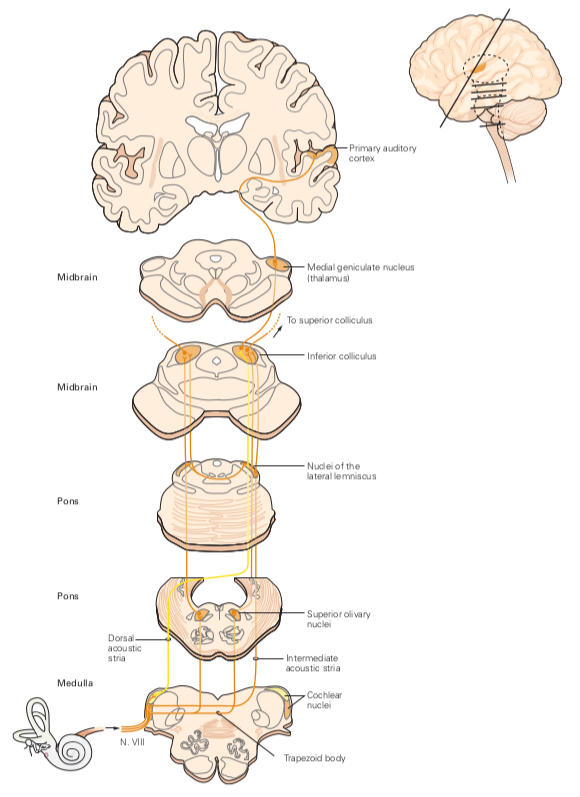
\includegraphics{pictures/auditory/hoerbahn_pathway.png}
    \caption[Hörbahn]{\textbf{Hörbahn} \\
    Die einzelnen Stationen der Hörbahn des Menschen von den Spiralganglionzellen in der Cochlea bis zum primären auditorischen Cortex anhand skizzierter Gehirnschnitte aus dem Kandel\textsuperscript{\cite[30]{kandel2013principles}} und einem Fließdiagramm}
    \label{fig:hoerbahn_pathway}
\end{figure}

\newpage
\noindent Efferente Fasern im Hörnerv innervieren die äußeren Haarzellen in der Cochlea, deren Aufgabe darin besteht die mechanische Auslenkung der Basilarmembran und der damit verbundenen Tektorialmembran zu verstärken oder zu unterdrücken. Infolgedessen kommt es zu einer verstärkten Selektivität und Sensibilität der Frequenzwahrnehmung\textsuperscript{\cite[29]{paxinos2014rat}}.

\subsubsection*{Nucleus cochlearis}

Die afferenten Ganglionzellen aus dem Hörnerv ziehen auf der Höhe der Medulla in den Hirnstamm und dort in das Kerngebiet den \textbf{Nucleus cochlearis} (\textbf{CN}). Dieser befindet sich  lateral auf der Höhe der Medulla (Abb.~\ref{fig:hoerbahn_pathway}) und bekommt nur Input aus dem Hörnerv der ipsilateralen Seite. Der NC besteht aus dem dorsalen Nucleus cochlearis (DCN) und dem ventralen Nucleus cochlearis (VCN), welcher wiederum in den anteroventralen (AVCN) und den posteroventralen (PVCN) Nucleus unterteilt wird\textsuperscript{\cite[29]{paxinos2014rat}}. Bei Ratten liegt der ventrale Nucleus cochlearis flach mediolateral an der Medulla, während der dorsale Nucleus cochlearis sich um den 'restiform body'\textsuperscript{\cite[29]{paxinos2014rat}}.
\\ \noindent Die auditorischen Nervenfasern verzweigen sich im Nucleus cochlearis in die verschiedenen Teile des CNs (Abb.~\ref{fig:Nucleus_cochlearis}B). Jede Faser gabelt sich in einen aufsteigen Ast zum AVCN und einen absteigenden Ast zum PVCN und DCN und leitet die Informationen an verschiedene Neurone in den Teilbereichen weiter\textsuperscript{\cite[29]{paxinos2014rat}}. Die Neuronen im ventralen Nucleus cochlearis codieren verschieden Eigenschaften, je nach Zelltyp. Im Allgemeinen schärfen sie das Timing und die Information aus dem Klangspektrum. 
\\

\begin{figure}[H]
    \centering
    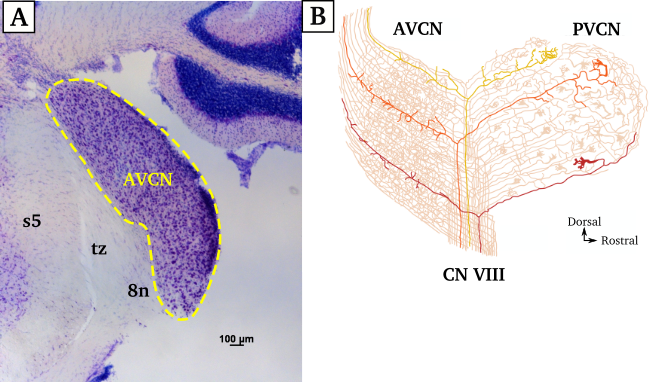
\includegraphics[width = \textwidth]{pictures/auditory/CN.png}
    \caption[Nucleus cochlearis]{\textbf{Nucleus cochlearis}\\
    \textbf{A}: Nissel-Färbung (N09\_1DL) der rechten Seite der Medulla. Es sind der anteroventrale Nucleus cochlearis (AVCN), der Trigeminus (s5), der Trapezkörper (tz) und der achte Hirnnerv (8n, Hörnerv) zu sehen. \textbf{B}: Verlauf der Nervenfasern aus dem achten Hirnnerv (CN VIII, 8n) im ventralen Nucleus cochlearis. Sowohl im anteroventralen (AVCN) als auch im posteroventralen (PVCN) Bereich des CNs werden die Fasern nach der Frequenz tonotopisch geordnet, von den tiefen Frequenzen (rot) ventral bis zu den hohen Frequenzen (gelb) im dorsalen Bereich. Abbildung B verändert nach Kandel \textsuperscript{\cite[31]{kandel2013principles}}}
    \label{fig:Nucleus_cochlearis}
\end{figure}

\newpage
Ein wesentlichen Teil spielt das Timing in der Weiterverarbeitung der Informationen in der oberen Olive, wohingegen die Verarbeitung des Klangspektrums in den ipsilateralen DCN, die ipsilaterale laterale obere Olive (LSO), den contralateralen ventralen Nucleus des lateralen Lemniscus und den contraleteralen Colliculus inferior projiziert wird. Ein Teil der Neuronen des Nucleus cochlearis projiziert in den contralateralen oberen paraoliven Nucleus (SPO) und den ventralen Nucleus des lateralen Lemniscus (VLL). Man nimmt an dass diese Bahnen bei der Verarbeitung von Störsignalen und Periodizität, sowie der Erkennung von Tonmustern eine Rolle spielt\textsuperscript{\cite[31]{kandel2013principles}}.  
\\\\
\noindent Der dorsale Nucleus cochlearis bekommt einerseits direkten Input von den Neuronen aus dem Hörnerv, zum anderen indirekten Input aus dem ventralen CN. Der dorsale CN integriert akustische  und somatosensorische Informationen um die Richtung der Schallquelle zu bestimmen\textsuperscript{\cite[31]{kandel2013principles}}.


\subsubsection*{Obere Olive}
Ein Großteil der Nervenzellen aus dem Nucleus cochlearis projizieren in die obere Olive. Die \textbf{obere Olive} (\textit{Nucleus olivaris superior}) ist für die Verarbeitung auditorischer Informationen wichtig und umfasst mehrere Kerngebiete. Innerhalb der Säugetiere variieren die Kerngebiete die unter dem Begriff obere Olive zusammengefasst werden. Drei Kerngebiete können bei fast allen Spezies gefunden werden: die \textbf{laterale obere Olive} (eng.: lateral superior olive, \textbf{LSO}), die \textbf{mediale obere Olive} (eng.: medial superior olive, \textbf{MSO}) und der \textbf{mediale Nucleus des Trapezkörpers} (eng.: medial nucleus of the trapezoid body, \textbf{MNTB}). Die LSO ist ein S-förmiges Kerngebiet im lateralen bereich der oberen Olive und ist durch ihre markante Struktur leicht zu erkennen (Abb.~\ref{fig:obere_Olive}). Die MSO liegt medial der LSO und ist bei Ratten ein kleineres Kerngebiet als beim Menschen. Der mediale Nucleus des Trapezkörpers (MNTB) befindet sich lateral in der oberen Olive\textsuperscript{\cite[29]{paxinos2014rat}}.

In Nagetieren, wie der Ratte, gibt es ein viertes, ausgeprägtes Kerngebiet, den \textbf{oberen paraoliven Nucleus} (eng.: superior paraolivary nucleus, \textbf{SPO}). Diese Kerngebiet befindet sich im dorsomedial Bereich der oberen Olive. Es bekommt die Informationen aus dem contralateralen Nucleus cochlearis und projiziert in den Colliculus inferior auf der ipsilateralen Seite\textsuperscript{\cite[29]{paxinos2014rat}}. Die SPO entschlüsselt besonders gut Muster in Tönen und Informationen in zeitlichen Mustern. Das spielt in der Wahrnehmung von Kommunikation ein Rolle, im Besonderen bei akustischen Schwebungen in Vokalisationen bei Tieren und Sprachsignalen\textsuperscript{\cite[29]{paxinos2014rat}}. 
\\\\
\begin{comment}
\textcolor{red}{Moreover, the SPO is particularly well suited to encode
rhythmic sound patterns and information on temporal
periodicity that is likely important for detection of com-
munication cues, such as the acoustic envelopes of animal
vocalizations and speech signals}
\end{comment}

\noindent Die drei Hauptkerne der oberen Olive spielen eine wichtige Rolle in der Verarbeitung von Schall. Aufgrund der Beschaffenheit der Cochlea werden dort nur die einzelnen Frequenzen kodiert, wobei dadurch keine Informationen über die Richtung der Schallquelle kodiert werden. Das Richtungshören wird in der oberen Olive integriert, durch die Verarbeitung der Informationen aus beiden Ohren. Sie ist damit die erste Schaltstelle in der Hörbahn die Input von der ipsilateralen und der contralateralen Seite, aus den jeweiligen Nuclei cochlearis, bekommt.
\newpage
\textbf{Mediale obere Olive}

\noindent Die mediale obere Olive (\textbf{MSO}) ist tonotopisch arrangiert. Die tiefen Töne werden dorsal in der MSO verarbeitet, wohingegen hohe Frequenzen im ventralen Part verarbeitet werden. Der Anteil der tiefen Töne ist proportional über repräsentiert in der MSO. Aus diesem Grund ist die MSO in der Ratte (Abb.~\ref{fig:obere_Olive}) klein, da Ratten im hochfrequenten Bereich hören.

Die mediale obere Olive erhält excitatorischen Input aus den beiden Nuclei, wobei die lateralen Dendriten der MSO, die Informationen aus dem ipsilateralen Nucleus cochlearis erhalten und die medialen Dendriten aus dem contralateralen Nucleus\textsuperscript{\cite[29]{paxinos2014rat}}. Da die Neuronen aus den Nuclei nur auf eine bestimmt Phase des Tons feuern (eng.: \textbf{phase-locking}), kann mit Hilfe der interauralen Zeitdifferenz und dem 'coincidence detection model' die Richtung, aus der der Ton kam, bestimmt werden\textsuperscript{\cite[31]{kandel2013principles}}.

Die Axone der MSO projizieren in den \textbf{dorsalen Nucleus des lateralen Lemniscus} (\textbf{DLL}) und in den \textbf{Colliculus inferioris} (\textbf{IC})\textsuperscript{\cite[29]{paxinos2014rat}}.
\\

\begin{comment}
It is tonotopically
organized with low frequency tones represented dorsally and high frequency tones ventrally, with most of the
nucleus devoted to low frequency tone
As mentioned, the MSO is diminutive
in that rat that has predominantly high frequency hear-
ing
MSO receives direct excitatory
input from both sides, although the inputs remain seg-
regated
The lateral dendrites receive input from the ipsilateral
side, the medial dendrites, from the contralateral side
(guinea pig: Smith, 1995). Collaterals of individual
axons from the spherical bushy cells travel different
distances in the rostro-caudal axis so that the collater-
als innervating the rostral MSO are shorter than those
innervating the caudal MSO in the cat
The proposed mechanism through which the MSO
analyzes interaural time differences is based on the coin-
cidence detection model of Jeffress\textsuperscript{\cite[29]{paxinos2014rat}}

The MSO projects mainly to the ipsilateral dorsal
nucleus of the lateral lemniscus (Kelly et al., 2009; cat:
Oliver and Shneiderman, 1989) and the central nucleus
of the inferior colliculus
\end{comment}


\begin{comment}
The LSO occupies a lateral position within the SOC
(Fig. 9). When viewed on transverse sections through
the brainstem, it appears as an S-shaped row of bipolar
neurons, with their dendrites oriented approximately
perpendicular to the long axis of the nucleus (Rietzel
and Friauf, 1998), which is also the tonotopic axis of
the nucleus: low-frequencies are represented laterally
and high-frequencies are represented medially

The LSO receives input from the VCA on both sides
(Figs. 3 and 5; Harrison and Irving, 1966b). The ipsi-
lateral input derives from spherical bushy cells and is
excitatory. Multipolar cells from the VCA whose axons
travel in the trapezoid body or in the intermediate
acoustic stria also innervate the LSO (Doucet
and Ryugo, 2003). Indirect input from the contralateral
VCA originates from globular bushy cells, which proj-
ect across the midline to the MTz

The MTz, in turn has a glycinergic inhibitory
projection to the LSO on the same side (cat: Moore and
Caspary, 1983; Saint-Marie et al., 1989; Adams and Mug-
naini, 1990). Consequently, LSO neurons are excited by
ipsilateral and inhibited by contralateral sounds (EI
units) and faithfully encode interaural intensity dif-
ferences in the high frequency range of audition

The LSO projects bilaterally to the central nucleus
of the inferior colliculus (Fig. 3; cat: Shneiderman and
Henkel, 1987). The ipsi- and contralateral projections are
provided by different cell classes. Most of the ipsilater-
ally projecting cells are glycinergic and probably inhibi-
tory.
The
contralaterally projecting cells are glycine-negative and
probably excitatory (Saint-Marie et al., 1989; Saint-Marie
and Baker, 1990). The LSO also innervates the dorsal
nucleus of the lateral lemniscus bilaterally
The MTz is located in the most medial part of the SOC

As mentioned above, the MTz receives input from
the VCA
\end{comment}

\begin{figure}[H]
    \centering
    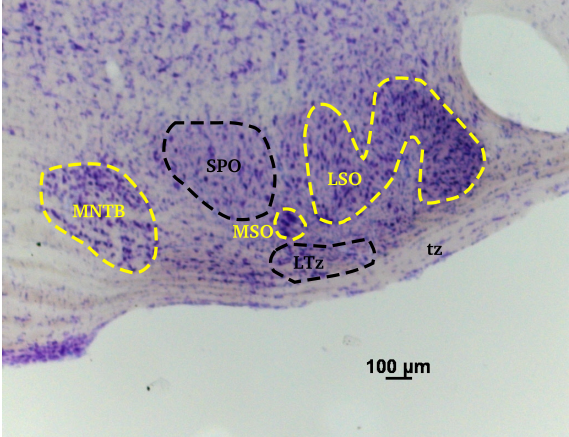
\includegraphics{pictures/auditory/obere_olive.png}
    \caption[Obere Olive]{\textbf{Obere Olive}\\
    Nissel-Färbung (N10\_1DL) der oberen Olive in der Pons. Mit den drei Hauptkernen mediale obere Olive (MSO), der lateralen oberen Olive (LSO) und dem medialen Nucleus des Trapezkörpers (MNTB) und dem für Nager speziellen oberen paraoliven Nucleus (SPO). Des weiteren liegt in der oberen Olive das Kerngebiet des lateralen Nucleus des Trapezkörpers (LTz) und der Trapezkörper (tz) selber, welcher die oberen Oliven beider Hirnhälften miteinander verbindet, befindet sich ventral des Komplex der oberen Olive.}
    \label{fig:obere_Olive}
\end{figure}

\newpage
\textbf{Laterale obere Olive}

\noindent Die laterale obere Olive (\textbf{LSO}) und der mediale Nucleus des Trapezkörpers (\textbf{MNTB}) zusammen, bilden eine Einheit, welche über die interaurale Intensitätsdifferenz das Richtungshören bei hohen Tönen, berechnet. 
 Die tonotopische Anordnung der LSO zieht sich entlang der S-Form von hohen Tönen medial bis zu tieferen Tönen lateral. Die LSO der Ratte ist im vergleich zum Menschen einiges größer, das Hängt unter anderem mit der Überrepresentation der hohen Töne in der lateralen oberen Olive zusammen und dem Hörbereich von Ratten.

Die LSO bekommt bilateralen Input. Der ventrale Nucleus cochlearis (VCN) der ipsilateralen Seite, leitet die Informationen excitatorisch an die LSO weiter. Vom contralateralen VCN werden die Informationen excitatorisch an den MNTB, der anderen Seite, über den Trapezkörper weiter gegeben. Von dort wird das Signal inhibitorisch an die LSO der selben Seite weiter geleitet.
Somit bekommen die Neuronen der LSO indirekten inhibitorischen Input aus dem contralateralen Nucleus cochlearis und excitatorischen Input aus dem ipsilateralen Nucleus cochlearis.

Die laterale obere Olive projiziert bilateral in den zentralen Nucleus des Colliculus inferior (\textbf{IC}), wobei auf die ipsilaterale Seite inhibitorisch projiziert wird und auf die contralaterale Seite excitatorisch.
Des weiteren projiziert ein Teil der Neuronen auch in den dorsalen Nucleus des lateralen Lemniscus (\textbf{DLL}) \textsuperscript{\cite[29]{paxinos2014rat}}.

\subsubsection*{Lateraler Lemniscus}

Die afferenten Nervenfasern aus der oberen Olive bilden den \textbf{Lemniscus lateralis} (\textbf{ll}) welcher über das Tegmentum pontis in den \textbf{Colliculus inferior} (\textbf{IC}) zieht und dort terminieren. Einige der Axone aus der oberen Olive terminieren in den \textbf{Nuclei des lateralen Lemniscus}. Des weiteren enden hier auch Nervenfasen die direkt aus den Nuclei cochlearis kommen \textsuperscript{\cite[10]{crossman2014neuroanatomy}}. 
Die Nuclei des lateralen Lemniscus unterteilen sich in den \textbf{dorsalen Nucleus des lateralen Lemniscus} (\textbf{DLL}) und den \textbf{ventralen Nucleus des lateralen Lemniscus} (\textbf{VLL}). Diese Unterteilung erfolgt anhand zweier funktional unterschiedlichen Systeme: die monoaurale Verarbeitung ventral und die binaurale Verarbeitung dorsal \textsuperscript{\cite[29]{paxinos2014rat}}. 
\\

\textbf{Ventraler Nucleus des lateralen Lemniscus}

Afferente Neuronen ziehen aus dem contralateralen ventralen Nucleus cochlearis (VCN) und dem ipsilateralen MNTB in den ventrale Nucleus des lateralen Lemniscus (\textbf{VLL}). Der VLL ist vorwiegend in der Verarbeitung von präzisen zeitlichen Informationen zuständig.
Es wird vermutet, dass die Zwischenstation in dem ventralen Nucleus als Relaisstation auf dem Weg zum Colliculus inferior funktioniert.
Der Nucleus ist aus isofrequenten Lamina aufgebaut und liegt in der Pons. Die Afferenzen zum Colliculus inferior sind ebenfalls tonotopisch arrangiert. Sie terminieren im zentralen Bereich des IC \textsuperscript{\cite[29]{paxinos2014rat}}.
\\

\begin{comment}
Afferent projections to the VLL arise mainly from
the contralateral VC (Figs. 3 and 5) and ipsilateral
MTz. Thus, it seems
that these cells would be suited to convey precise and
secure temporal information (Nayagam et al., 2005,
2006). Both primary-like and chopper responses have
been observed (Nayagam et al., 2005, 2006) after stim-
ulation with pure tones, consistent with the idea that
globular and multipolar cells take part in the projection
(cat: Smith et al., 1991). Because of these connections,
the VLL may be acting as a mere relay station in the
projection to the inferior colliculus, but more probably
these responses may also be generated de novo within
the VLL as suggested by others (Zhao and Wu, 2001;
Nayagam et al., 2005, 2006). The MTz projects to the
dorsal portion of the complex (Kelly et al., 2009; cat:
Glendenning et al., 1981; Spangler et al., 1985). Other
sources of projections to the VLL are the periolivary
nuclei, including the ipsilateral SPO (Kelly et al., 2009;
Saldaña et al., 2009). Many auditory neurons have
extensive local connections in addition to their main
projection, e.g., cochlear nuclear complex: Doucet and
Ryugo (1997, rat) or inferior colliculus: Malmierca
(1991, rat); the same seems to hold true for the VLL
neurons in rats (Zhao and Wu, 2001).

These authors also
demonstrate that the neurons form a partly continuous
laminar structure and that VLL projections to the IC are
topographically organized with respect to the sound fre-
quency. Thus, Merchán and Berbel (1996) concluded that
the rat VLL is a single nucleus, composed of isofrequency
laminae extending through the whole dorsoventral and
rostrocaudal length of the complex.

it is also clear that virtually all cells in the rat VLL
project to the central nucleus of the inferior colliculus, as
in the cat (Whitley and Henkel, 1984).
\end{comment}


\textbf{Dorsaler Nucleus des lateralen Lemniscus}

Der dorsale Nucleus des lateralen Lemniscus (\textbf{DLL}) liegt oberhalb des ventralen Nucleus des lateralen Lemniscus in der Pons. Er bekommt bilateralen Input. Von der contralateralen Seite projizieren die Neuronen aus dem ventralen Nucleus cochlearis (VCN) und dem DLL, von der ipsilateralen Seite projizeren afferent Nervenfasern aus der MSO, SPO und dem VLL. Von beiden Seiten ziehen in den dorsalen Nucleus Afferenzen aus der lateralen oberen Olive (LSO).
Aufgrund der vielen Verbindungen zu tiefer liegenden Kernen wie der LSO und MSO spielt der dorsale Nucleus eine Rolle beim Richtungshören. Läsionen im DLL bewirken ein Defizit im Richtungshören und eine Ungenauigkeit in der räumlichen Hörschärfe. 
Der DLL projiziert über den lateralen Lemniscus in beide Colliculi inferior (IC) und über die Probst commisur in den gegenüberliegenden dorsalen Nucleus des lateralen Lemniscus
\textsuperscript{\cite[29]{paxinos2014rat}}.

\begin{comment}
The DLL is a distinctive group of neurons embedded
within the dorsal part of the lateral lemniscus (Fig. 3) that
projects bilaterally to the inferior colliculus. In the rat,
the DLL is cube-shaped
he DLL is a distinctive group of neurons embedded
within the dorsal part of the lateral lemniscus (Fig. 3) that
projects bilaterally to the inferior colliculus. In the rat,
the DLL is cube-shaped
In con-
trast to the VLL, the DLL receives input from both ears,
and it projects to both inferior colliculi (Fig. 3) and also
to its homolog on the opposite side (Fig. 3) through the
commissure of the lateral lemniscus (cll) or Probst’s com-
missure
The DLL receives input from both ears, contralater-
ally from the VC and DLL, ipsilaterally from the MSO,
SPO and VLL, and bilaterally from the LSO

Function

An essential issue in the central auditory system con-
cerns how the origin of a sound is localized. Where func-
tions such as pitch or intensity coding can be performed
by one ear alone, the accurate localization of a sound
requires the use of both ears and depends on the com-
parison of the sounds they receive (for review, see Yin and
Chan, 1988). The afferent and efferent connections of the
DLL suggest that this nucleus plays an important role in
binaural processing (e.g., sound localization).

Also, behavioral studies have
shown deficits in sound localization and a reduction in
spatial acuity after lesions of DLL
\end{comment}


\begin{figure}[H]
    \centering
    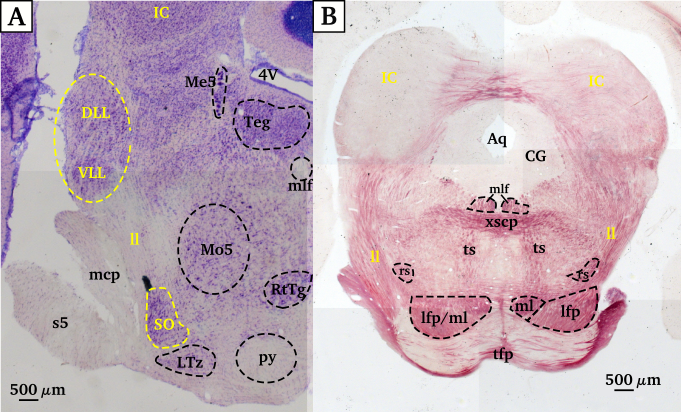
\includegraphics[width = \textwidth]{pictures/auditory/lateral_lemniscus.png}
    \caption[Der Lateraler Lemniscus und seine Kerne]{\textbf{Der Lateraler Lemniscus und seine Kerne}\\ 
    Verlauf des lateralen Lemniscus und die Lage seiner Kerne in der Nissel-Färbung (N11\_4P) und der Faser-Färbung (N13\_4P). Die Schnittebenen sind 1200~$\mu$m auseinander.\\
    \textbf{A}: Nissel-Färbung (N11\_4P) auf der Höhe der Pons, erkennbar am vierten Ventrikel (4V).
    Der laterale Lemniscus verbindet die obere Olive (SO) mit dem Colliculus inferior (IC). Einige der Verbindungen sind über den dorsalen (DLL) oder den ventralen (VLL) Nucleus des lateralen Lemniscus zwischen geschaltet. 
    Des weiteren sind der Trigeminus (s5) und der Nucleus des mesencephalischen Tracts des Trigeminus (Me5) aus der Somatosensorik und der motorische Nucleus des Trigeminus (Mo5) aus der Motorik zu sehen. 
    Weitere Kerngebiete und Fasertrakte sind: lateraler Nucleus des Trapezkörpers (LTz), mittlerer cerebellarer Penduncle (mcp), medialer Fasciculus longitudinalis (mlf), Pyramidenbahn (py), reticulotegmentaler Nucleus der Pons (RtTg), Tegmentum (Teg)\\
    \textbf{B}: Verlauf des lateralen Lemniscus (ll) bis in den Colliculus inferior (IC) im Mesencephalon. Das zentrale Höhlengrau (CG) und das Aquädukt (Aq) sind zwei prominente Strukturen die im Mesencephalon liegen. Des weiteren sind folgende Fasertrakte zu sehen: Fasciculus longitudinalis der Pons (lfp), medialer Lemniscus (ml), medialer Fasciculus longitudinalis (mlf), rubrospinaler Tract (rs), transversale Fasern der Pons (tfp), tectospinaler Tract (ts), Kreuzung (decussation) des oberen cerebellaren Peduncles (xscp)}
    \label{fig:lateraler_lemniscus}
\end{figure}

\newpage
\subsubsection*{Colliculus inferior und Nucleus geniculatum mediale}

Die Fasern des lateralen Lemniscus ziehen in den \textbf{Colliculus inferior} (\textbf{IC}) und terminieren dort. Er liegt bei der Ratte sichtbar im dorsalen Bereich auf dem Mittelhirn, caudal vom Colliculus superior und bildet mit diesem zusammen die Vierhügelplatte \textsuperscript{\cite[29]{paxinos2014rat}}. \textcolor{red}{verweis auf den colliculus im teil von jule} 
Der IC integriert nahezu die gesamten Informationen aus den tiefer liegenden auditorischen Kerngebieten des Hirnstamms. Das macht ihn zu einem großen Integrationszentrum für die Verarbeitung des Richtungshören und auch für Tonhöhen \textsuperscript{\cite[29]{paxinos2014rat}}.

Vom Colliculus inferior aus geht die Hörbahn in den \textbf{medialen Kniehöcker} (\textit{Corpus geniculatum mediale}). Eine weitere Bahn führt direkt in den Colliculus superior (SC), welcher bei reflexiven Bewegungen zur Orientierung eine Rolle spielt. Desewgen nimmt man an dass, im SC eine auditorische Karte der Umgebung erstellt wird. Eulen sind bekannt für solche Karten die eine 3D Ansicht der Geräusche um sie herum sind. Zusammen mit Karten aus dem visuellen System und dem somatosensorischen System spielt der Colliculus superior eine entscheidende Rolle in motorischen Orientierung beim greifen nach Gegenständen \textsuperscript{\cite[31]{kandel2013principles}}.
\\
Der mediale Kniehöcker (\textbf{MG}) liegt auf der posterolateralen Seite des Thalamus. Es ist eine runde Erhebung lateral-ventral des Colliculus superior. Es ist das letzte Integrationszentrum in der auditorischen Hörbahn vor dem Cortex. Es bekommt Input aus dem Colliculus inferior (IC) über das \textit{Brachium colliculi inferioris} und absteigende Fasern aus dem auditorischen Cortex und dem reticularen Nucleus terminieren im MG. Afferente Nervenfasern aus dem medialen Kniehöcker ziehen ipsilateral in den auditorischen Cortex \textsuperscript{\cite[29]{paxinos2014rat}}. Der mediale Kniehöcker ist in drei Untereinheiten aufgeteilt: den ventralen, den dorsalen und den medialen Part. Der ventrale mediale Kniehöcker hat eine rein akustische Funktion, wohingegen der dorsale Part bei akustischer Aufmerksamkeit mitwirkt und der mediale Part bei multisensorischer Erregung und emotionalem akustischen Lernen eine Rolle spielt \textsuperscript{\cite[29]{paxinos2014rat}}.

\begin{figure}[H]
    \centering
    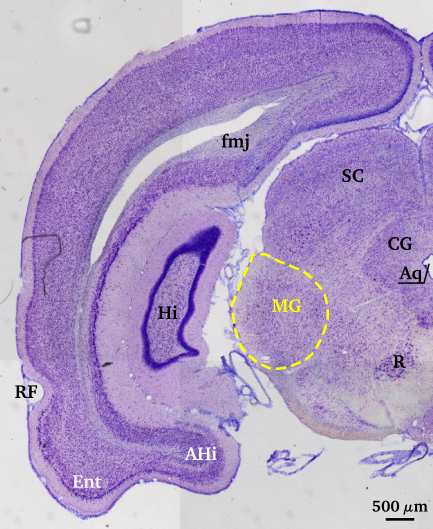
\includegraphics{pictures/auditory/MG.png}
    \caption[Corpus geniculatum mediale]{\textbf{Corpus geniculatum mediale}\\
    Das Corpus geniculatum mediale (MG) liegt im Mesencephalon lateral-ventral des Colliculus superior (SC). Das Aquädukt (Aq) wird vom zentralen Höhlengrau (CG) umgeben und unterhalb liegt der Nucleus ruber (R), welcher ebenfalls im Mesencephalon liegen. Der Cortex liegt um das Mesencephalon herum. Dazu zählen der Archicortex (AHi) der Cortex entorhinalis (Ent), Forceps major des Corpus callosum (fmj) un der Hippocampus (Hi). Nissel-Färbung (N16\_3P)}
    \label{fig:MG}
\end{figure}

\begin{comment}
The inferior colliculus (IC, Figs. 12–19) is visible on
the dorsal surface of the midbrain immediately caudal
to the superior colliculus (Figs. 3 and 12). 
The IC receives fibers from lower and higher auditory
centers (Figs. 3, 5, and 14) as well as from non-auditory
structures

Obgleich es andere Routen mit weiteren zwischengeschalteten Relais von
den Cochleariskernen zum Colliculus inferior gibt, konvergieren sämtliche aufsteigenden
Hörbahnen auf den Colliculus inferior. Die Neuronen im Colliculus inferior senden Axone
zum Corpus geniculatum mediale (CGM) des Thalamus, das seinerseits in den auditori-
schen Cortex projiziert. \textsuperscript{\cite[11]{neurowissenschaften_baer}}

Auditory information ascends to the cerebral cortex
through the thalamus. Neurons of the inferior collicu-
lus project to the medial geniculate body, where prin-
cipal cells in turn project to the auditory cortex. The
pathways from the inferior colliculus include a lemnis-
cal or core pathway and extralemniscal or belt path-
ways. Descending projections from the auditory cortex
to the medial geniculate body are prominent both ana-
tomically and functionally. \textsuperscript{\cite[31]{kandel2013principles}}

Central nucleus neurons project to the thalamus and
also to the external cortex of the inferior colliculus and
the nucleus of the brachium of the inferior colliculus,
both of which then project to the superior colliculus (or
the optic tectum in birds).
The superior colliculus is critical for reflexive ori-
enting movements of the head and eyes to acoustic and
visual cues in space. By the time they reach the supe-
rior colliculus, binaural sound cues and the monaural
spectral cues that underlie mammalian sound localiza-
tion merge to create a spatial map of sound, an audi-
tory map, in which neurons are unambiguously tuned
to specific sound directions. This convergence is criti-
cal, for the binaural level and timing differences alone
cannot unambiguously code for a single position in
space. The spectral cues that provide information about
vertical location are essential. Different locations in the
vertical plane can give rise to identical interaural time
or intensity differences. Such a spatial map is formed
both in birds and in some mammals (Figure 31–8). In
ferrets and guinea pigs topographic representations of
the location of sound in the horizontal plane are found
in the external cortex and the nucleus of the brachium
of the inferior colliculus.
Within the superior colliculus the auditory map
is congruent with maps of visual space and the body
surface. Unlike the visual and somatosensory maps,
the auditory map is computed from a combination
of cues that identify the specific position of a sound
source in space, and is not based on the peripheral
receptor surface.
Auditory, visual, and somatosensory neurons in the
superior colliculus all converge on output pathways in
the same structure that controls orienting movements
of the eyes, head, and external ears. The motor circuits
of the superior colliculus are mapped with respect to
motor targets in space, and are aligned with the sen-
sory maps. Such sensory-motor correspondence facili-
tates the sensory guiding of movements. \textsuperscript{\cite[31]{kandel2013principles}}

The medial geniculate body (MG; Figs. 20–24) lies on
the posterolateral surface of the thalamus (see Thalamus,
Chapter 16) as a rounded eminence, lateral and ventral
to the superior colliculus, marking the rostral pole of the
brachium of the IC. It represents the main auditory cen-
ter of the thalamus and is the last center for auditory pro-
cessing before inputs reach the auditory cortex

These fibers enter
the MG via the brachium of the inferior colliculus (Figs. 3
and 18). The MG also receives descending fibers from
the auditory cortex (Hazama et al., 2004; Kimura et al.,
2005, 2007a; Smith et al., 2007) and reticular thalamic
nucleus (Rt; Shosaku and Sumitomo, 1983; Kimura et al.,
2007b) (Figs. 24 and 29). The rat MG differs from the IC
in several respects (Winer, 1991, 1992; Winer et al., 1996)
in that its afferent projections are primarily ipsilateral.
MG targets include the auditory cortex as well as sub-
cortical limbic forebrain structures

he MG contains three main divisions (Figs. 3 and
20): ventral (MGV), dorsal (MGD) and medial (MGM),
each defined on the basis of cytoarchitecture and fiber
connections (

that the MGV has a
purely acoustic function, while the MGD is involved in
acoustic attention, and the MGM and remaining poste-
rior paralaminar thalamic nuclei are involved in multi-
sensory arousal and emotional auditory learning \textsuperscript{\cite[29]{paxinos2014rat}}

\end{comment}


\subsubsection*{Primärer auditorischer Cortex}

Die primäre Hörrinde auch \textbf{primärer auditorischer Cortex} \index{Auditorischer Cortex! primärer} genannt erhält akustische Informationen aus der bisher beschriebenen Hörbahn. Aufgrund der Verschaltung der Hörbahn bekommt sowohl die linke als auch die rechte Gehirnhälfte und das dort liegende primäre auditorische Areal, Informationen aus beiden Ohren. Einige Eigenschaften wie die interaurale Zeitdifferenz und die interaurale Intensitätsdifferenz, berechnet in der oberen Olive, werden hier zum entgültigen Richtungshören integriert. 

Die Fasern aus dem medialen Kniehöcker enden in tonotopisch Anordnung, tiefe Frequenzen mehr anterolateral und hohe Frequenzen mehr posteromedial beim Menschen, in der primären Hörrinde \textsuperscript{\cite[9.9]{trepel2011neuroanatomie}}. Die Fasern aus der Hörbahn enden in den Heschl-Querwindungen des Temporallappens. Der primäre auditorische Cortex (Brodmann's Areal 41 und 42) liegt im Temporallappen, genauer gesagt im oberen Gyrus des Temporallappens, versteckt im \textit{Sulcus lateralis} \textsuperscript{\cite[13]{crossman2014neuroanatomy}}. 

Die primären Hörrinde ist für das interpretationsfreie bewusst werden von wahrgenommenen auditorischen Signalen veranwortlich. Das heißt im Klaren, wenn man im primären auditorischen Cortex reizt, werden Laute und Muster wahrgenommen, aber keine Melodien oder Sprache. Die Zusammensetzung einzelner Laute zu Srache geschieht erst in der sekundären Hörrinde \textsuperscript{\cite[9.9]{trepel2011neuroanatomie}}.

\begin{comment}
fur die inter-
pretationsfreie Bewusstwerdung der auditarischen Impulse
aus dem hmenohr verantwortlich. Bei (experimenteller) Rei-
zung der primären Hörrinde werden dementsprechend immer
nur einzelne Laute oder Lautmuster mtterschiedlicher Fre-
quenz, niemals aber Wörter oder Melodien wahrgenommen.
Die sinnvolle Verknüpfung dieser Laute zu Wörtem oder
schließlich Sätzen und dergleichen erfolgt erst in der sekundä-
ren Hörrinde, die das Ziel der effurenten Bahnen der primären
Hörrinde ist.

The lateral surface of the temporal lobe is divided into
superior, middle and inferior temporal gyri, which run
parallel to the lateral fissure. Within the superior temporal
gyrus is located the primary auditory cortex (Brodmann’s
areas 41 and 42). More exactly, most of this functional zone
lies in the superior bank of the gyrus, normally hidden within
the lateral fissure \textsuperscript{\cite[13]{crossman2014neuroanatomy}}.

Die primäre Hörrinde er-
hält somit akustische Informationen aus beiden Cochleae,
was sich klinisch bei einer einseitigen Schädigung der Hör-
bahn positiv auswirkt. Weiterhin wird durch die Konver-
genz der Hörinformation beider Seiten (die z. T. bereits auf
Hirnstammebene erfolgt, s. o.) das Richtungshören ermög-
licht. 

Die Hörbahn ist die wichtigste .Aflerenz des auditorischen
Kortex. Die Hörbahnfasern enden hier in tonotopischer An-
ordnung, d. h., jede Tonfrequenz hat ihren eigenen Terminati-
onsoft in der primären Hörrinde (tiefe Frequenzen mehr ante-
rolateral, hohe mehr posteromedial). Als primärer Endigmtgs-
ort der Hörbahn sind die Heschl-Quenvindungen (analog zur
primären somatasensiblen oder visuellen Rinde) fur die inter-
pretationsfreie Bewusstwerdung der auditarischen Impulse
aus dem hmenohr verantwortlich. Bei (experimenteller) Rei-
zung der primären Hörrinde werden dementsprechend immer
nur einzelne Laute oder Lautmuster mtterschiedlicher Fre-
quenz, niemals aber Wörter oder Melodien wahrgenommen.
Die sinnvolle Verknüpfung dieser Laute zu Wörtem oder
schließlich Sätzen und dergleichen erfolgt erst in der sekundä-
ren Hörrinde, die das Ziel der effurenten Bahnen der primären
Hörrinde ist.
\textsuperscript{\cite[9.9]{trepel2011neuroanatomie}}
\end{comment}

\subsubsection*{Sekundärer auditorischer Cortex und cortico-corticale Verbindungen}

Der \textbf{sekundäre auditorische Cortex} \index{Auditorischer Cortex! sekundärer} liegt lateral der primären Hörrinde und nimmt die Brodmann Areale 42 und 22 ein. Der Cortex bekommt den Input von der primären Hörrinde. Dabei ist die Verarbeitung auf den beiden Hemisphären unterschiedlich. Bei Rechtshändern wird auf der linken Hirnhälfte der sekundäre auditorische Cortex auch \textbf{Wernicke-Areal} \index{Wernicke-Areal} genannt. Das Wernicke-Areal (Abb.~\ref{fig:Wernicke}) integriert die auditorische Informationen für das Verständnis von Sprache. Der sekundäre auditorische Cortex integriert die auditorischen Informationen auf eine mehr rationale Weise. Die Hemisphäre auf der die Sprache verarbeitet wird ist die dominante Hemisphäre. Dies seht im Gegensatz zur Verarbeitung des sekundären auditorischen Cortex auf der rechten Hemisphäre bei Rechtshändern. Es werden mehr 'nicht-rationale' Komponenten verarbeitet. Dazu zählt das erkennen und Verständnis von Musik. Man nennt die Hemisphäre auch die nicht-dominante Hemisphäre. Für Rechtshänder trifft die oben genannte Einteilung in dominante Hemisphäre links und nicht-dominante Hemisphäre rechts zu. Für Linkshänder ist die Einteilung nicht so klar und somit kann die nicht-dominante Hemisphäre rechts oder links sein \textsuperscript{\cite{trepel2011neuroanatomie}}.

Einen weiteren Input bekommt der sekundäre auditorische Cortex vom Gyrus angularis, welcher wiederum mit dem sekundären visuellen Cortex verknüpft ist. Diese Verbindung spielt eine Rolle bei dem Verständnis von gelesener Sprache. Die gesehene Schrift oder das Benennen von gesehenen Gegenständen wird im Wernicke-Areal mit dem Sprachverständnis verknüpft. 

Das Wernicke-Areal ist über den \textbf{Fasciculus arcuatus} \index{Fasciculus arcuatus} mit dem \textbf{Broca-Areal} \index{Broca-Areal} verknüpft. Das Broca-Areal (Brodmanm Areal 44 und 45) liegt im Frontallappen und gehört zum Motorcortex. Dieses Konstrukt wird \textbf{Wernicke-Gerschwind Modell} \index{Wernicke-Gerschwind Modell} genannt und verbindet das Sprachverständnis im Wernicke-Areal mit der Sprachproduktion im Broca-Areal. Einige Zeit nahm man an, dass diese Verbindung (Fasciculus arcuatus) nur unidirektional ist, Studien belegten aber, dass die Verbindung in beide Richtungen läuft und auch noch weitere Gehirnareale an dem Verständnis und der Produktion von Sprache beteiligt sind \textsuperscript{\cite[60]{kandel2013principles}}.

\begin{figure}[H]
    \centering
    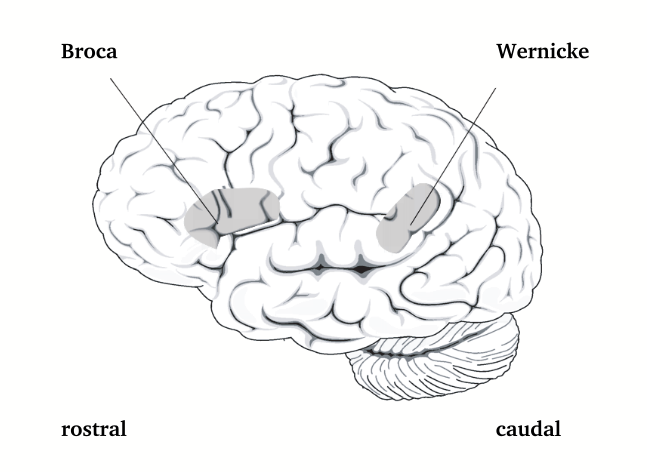
\includegraphics{pictures/auditory/Wernicke.png}
    \caption[Wernicke-Areal]{\textbf{Wernicke-Areal}\\ 
    Wernicke-Areal und Broca-Areal auf der dominanten (linken) Hemisphäre. Die Verbindung der Beiden Areale (Fasciculus arcuatus) ist nicht abgebildet, verläuft aber um den Sulcus lateralis herum.
    Abbildung veränder nach \url{https://www.nidcd.nih.gov/health/aphasia}}
    \label{fig:Wernicke}
\end{figure}


\begin{comment}
Dieses Kortexareal nimmt die Areae 42 und 22 nach Brodmann
ein (- Abb. 9.37) m1d grenzt somit lateral direkt an die pri-
märe Hörrinde in den Heschl-Quenvindungen an, aus der es
auch den Großteil seiner Afferenzen erhält. Hier erfallren die
auditarischen Impulse der primären Hörrinde eine interpreta-
tive Verarbeitung. Die Laute werden als Wörter, Melodien,
Geräusche e-rkannt. Interessanterweise nehmen die sekundä-
ren Hörrinden beider Hemisphären dabei einen unterschiedli-
chen Stellenwert ein:
In der dominanten Hemisphäre werden auditarische Im-
pulse mehr rational integriert einschließlich des Verständ-
nisses der Sprache. Deswegen wird die sekundäre Hörrinde
hier auch als sensorisches Spra.chzentrun1 (Wemicke) be-
zeichnet, auch wenn am Sprachverständnis noch weitere
Regionen des Gehirns beteiligt sind.
In der nicht-dominanten Hemisphäre vird in der sekml-
dären Hörrinde offensichtlich mehr die ,,nicht-rationale"
Komponente des Gehörten verarbeitet, z. B. das Erkennen
und Verständnis von Musik. Definitionsgemäß ist diejenige
Hemisphäre dominant, in der motorisch m1d sensorisch die
Sprache verarbeitet wird (bei Rechtshändern die linke, bei
Linkshändern die rechte oder die linke).
Diese Zuordnung der dominanten und nicht-dominanten He-
misphäre zu mehr verbal-rationalen und mehr nonverbal-mu-
sischen Integrationsvorgängen gilt nicht nur für die sekundäre
Hörrinde, sondern auch für viele andere Kortexareale, darf
aber nicht zu dogmatisch und streng interpretiert werden.

Afferent ist die sekundäre Hörrinde neben der primären Hör-
rinde auch intensiv mit dem Gyrus a.ngularis ( >- Abb. 9.30)
verbtmden, der eine zentrale Bedeutung bei der Verknüpfung
von Gesehenem m1d der Sprache hat. Dies spielt z. B. beim Vorgang des Schreibens oder Lesens eine herausragende Rolle:
Der Gyrus angularis erhält seine Impulse vor allem aus dem
sekundären visuellen Kortex. Diese Infonuation der als Schrift
erkannten Impulse aus der Sehrinde wird dann vom Gyrus an-
gularis an das W ernicke-Sprachzentrum weitergesandt und
dort mit dem Sprachverständnis verknüpft. Auch bei anderen
Funktionen, z. B. beim begrifflichen Benennen von gesehenen
Gegenständen, gilt das gleiche Prinzip. \textsuperscript{\cite{trepel2011neuroanatomie}}
\end{comment}

\newpage
\subsection{Sehbahn}

Der visuelle Sinn ist 

Was ist das besondere an diesem Sinn, welche generellen Besonderheiten gibt es - inverted vs verted eye, 


\subsubsection*{Das Auge}
\index{Auge}
Das Auge ist das primäre Sehsinnesorgan. Dort befinden sich die lichtbrechenden Strukturen wie die Cornea \index{Cornea} und die Linse, \index{Linse} welche die Abbildungsqualität auf dem Auge bestimmen. Die Retina ist die Zellstruktur, in der die Lichtimpulse durch die Photorezeptoren wahrgenommen werden und das Signal über die Bipolarzellen zu den Ganglionzellen leiten. Welche dann wiederum die Informationen bis ins Gehirn weiter geben.
Das Auge bei Säugetieren ist ein invertes Linsenauge, \index{Linsenauge} das sich zu Teilen aus dem Diencephalon entwickelt. 
\\
\\
Das Auge bei Säugetieren ist eine Struktur die sich im Laufe der embrionalen Entwicklung aus Zellen des Ektoderms und des Mesoderms entwickeln. Bei der Entwickung der der Neurula, differenzieren Zellen im dorsalen Bereich zu Neuroektodermzellen \index{Neuroektoderm} (Abb.~\ref{fig:eye_neurulation}~A). Welche dann im weiteren Verlauf der Entwicklung zur Neuralplatte und dann zum Neuralrohr sich entwickeln (Kapitel~\ref{subsec:Neurulation}). 
Es wird angenommen, dass in einem frühen Stadium der evolutionären Entwickung unserer Vorfahren, diese freischwimmende Lebewesen waren, deren ursprüngliche Photorezeptoren in 'diesem Streifen reaktiver Zellen' lagen. Diese waren dann auswärts gerichtet wie bei das auch im Aufbau des Linsenauges bei Weichtieren. Bei der Einstülpung des Ektoderms bei der Neurulation liegen die Photorezeptoren dann abgewandt vom Licht auf der Innenseite des Auges. 

Bei der Entwicklung des Embryos, nach der Einstülpung zum Neuralrohr entwickeln sich die Gehirnbläschen(Abb.~\ref{fig:eye_neurulation}~C). Aus dem Diencephalon stülpt sich ein Teil des Ektoderms aus und entwickelt sich zum optischen Vesikel (Abb.~\ref{fig:eye_neurulation}~D), welcher sich dann zur Augengrube \index{Augengrube} entwickelt. Aus dieser wiederum entsteht dann die Retina. Die Linse das Auges entwickelt sich während dessen ebenfalls aus ektodermalen Zellen. Diese werden durch die Zellen des optischen Vesikels \index{Vesikel! optischer} im Mesoderm induziert, es entsteht eine sogenannte Linsenplakode \index{Linsenplakode} (Abb.~\ref{fig:eye_neurulation}~E), welcher sich einstülpt und dann abspaltet (Abb.~\ref{fig:eye_neurulation}~F~\&~G).

Der Rest des Auges entwickelt sich aus dem Mesoderm. \textsuperscript{\cite[16]{smith2008biology}}

\begin{figure}[H]
    \centering
    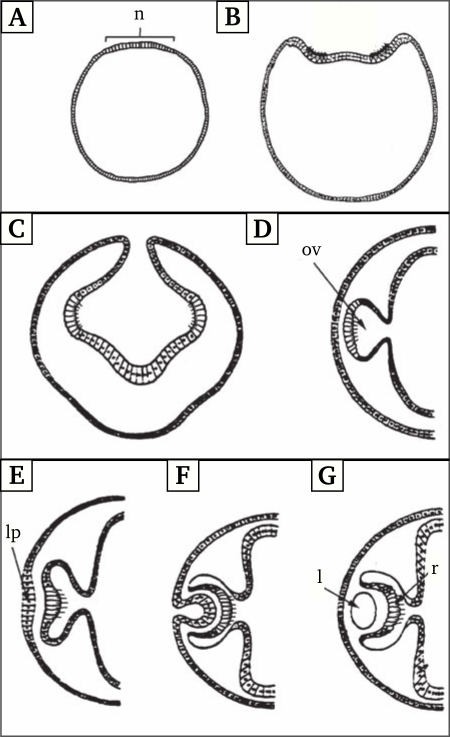
\includegraphics{pictures/visual/Eye_Neurulation.png}
    \caption[Embryonale Entwicklung des Auges]{\textbf{Embryonale Entwicklung des Auges}\\
    \textbf{A}: Neurula mit Neuroektodermzellen (n). \textbf{B}: Blastula mit ausgebildeter Neuralplatte. \textbf{C}: Einstülpung zum Neuralrohr. \textbf{D}: Entwichllung des optischen Vesikels (ov) aus dem Diencephalon. \textbf{E}: Migration der Ektodermzellen ins Mesoderm für die Bildung der Linse (Linsenplakode, lp). \textbf{F}: Bildung der Augenbrube und Einstülpung der Linsenplakode. \textbf{G}: Linse (l) und Photorezeptoren (r), auf der abgewandten Seite des Lichts\\
    Abbildung nach Biology of Sensory System, Smith \textsuperscript{\cite[16]{smith2008biology}}}
    \label{fig:eye_neurulation}
\end{figure}


\begin{comment}
The retina originates in a circuitous manner, inter-
nally, from the central nervous system (CNS). We
shall see that it is because of this convoluted route
of origin that it is ‘inverted’. The photoreceptors end
up facing away from the incoming light.
The vertebrate eye develops partly from mesoder-
mal tissue and partly from ectodermal tissue. The ec-
todermal tissue forms the retina and the non-neural
epithelial continuation of the retina which covers the
ciliary body and the posterior of the iris. Ectoderm
also forms the lens. Mesodermal tissue forms all the
rest. It has often been said that the retina is a por-
tion of the brain pushed to the exterior. We shall
see the sense of this proposition when we follow its
embryological origin. \textsuperscript{\cite[16]{smith2008biology}}

Figure
Series of transverse sections to show the em-
bryological origin of retina and lens. (a) Early embryo (neurula)
in which a strip of neurectoderm differentiates on the dorsal
surface; (b) Neurectoderm sinks inwards and two hollows, the
foveolae opticae, appear; (c) Neural tube beginning to form;
(d) Evagination of optic vesicle; (e) Optic cup beginning to form
and lens beginning to be induced from the overlying ectoderm.
(f) Optic cup continuing to invaginate and lens continuing to
form. (g) Optic cup almost fully formed; lens detached from
overlying ectoderm. Note the position of the photoreceptor out-
ersegments throughout. f = foveolae opticae; l = lens; l.p. =
lens placode; n = neurectoderm; o.v = optic ventricle; r = pho-
toreceptor outersegments.
\end{comment}

\subsubsection*{Die Retina}

\index{Retina}

Die Retina ist in laminaren Schichten aufgebaut (Abb.~\ref{fig:retina}).
Wie schon im vorhergehenden Abschnitt erwähnt, ist die Retina invers zum einfallenden Licht aufgebaut. Dies stellt kein Problem dar, da die Netzhautzellen (Ganglienzellen, Bipolarzellen, Amakrinzellen und Horizontalzellen) relativ transparent sind. Das Licht trifft zuerst auf die Schicht der \textbf{Ganglienzellen}. \index{Ganglienzellen} Deren Aufgabe ist die Signaltransduktion aus der Retina ins Gehirn. In der nächsten Schicht (innere plexiforme Schicht) liegen die synaptischen Verbindungen von den Ganglienzellen, den \textbf{Biploarzellen} \index{Bipolarzellen} und \textbf{Amakrinzellen}. \index{Amakrinzellen} Letzter beiden haben ihre Zellkörper in der inneren Körnerschicht. In der inneren Körnerschicht liegen auch die Zellkörper der \textbf{Horizontalzellen}. \index{Horizontalzellen} In der nächsten Schicht sind die Horizontalzellen mit den Bipolarzellen und den Photorezeptorzellen verbunden. Die Zellkernen der \textbf{Photorezeptorzellen} \index{Photorezeptorzellen} liegen in der äußeren Körnerschicht.Die Außensegmente der Photorezeptorzellen sind die eigentliche Struktur der Photorezeptoren, die das eintreffende Licht verarbeiten. Die Enden der Außensegmente sind im \textbf{Pigmentepithel} \index{Pigmentepithel} eingebettet. Dieses hat die Aufgabe Aufgabe der Erneuerung der Photorezeptoren und der Photopigmente. Des weiteren absorbieren die Pigmentepithelzellen sämtliches Licht das die Netzhaut durchdringt. Aus diesem Grund wird die Streuung auf ein Minimum reduziert und erhöht somit die Schärfe des Bilds. \textsuperscript{\cite[10]{neurowissenschaften_baer}}
\\
\\
Die Photorezeptoren werden in \textbf{Stäbchen} \index{Stäbchen} und \textbf{Zäpfchen} \index{Zäpfchen} unterschieden. Die Stäbchen ermöglichen ein Hell-Dunkel-Sehen, aufgrund ihrer niedrigen Toleranzschwelle. Bei den Zäpfchen unterscheidet man zwischen den blau-sensitiven, grün-sensitiven und rot-sensitiven Zäpfchen. Die Unterscheidung erfolgt anhand des Absorbtionsspektrum des einzelne Zäpfchens. Die Verteilung der Stäbchen und Zäpfchens über die Retina ist nicht konstant. Im Randbereich der Retina sind mehr Stäbchen, während es zur \textbf{Fovea} \index{Fovea} weniger werden. Die Fovea selber ist der Bereich der Retina in dem es keine Stäbchen gibt, sondern nur Zäpfchen. Außerdem sind in diesem auch die anderen Zellschichten zur Seite verdrängt. Die Fovea ist der Bereich mit dem schärfsten Sehen. \textsuperscript{\cite[10]{neurowissenschaften_baer}}

\begin{figure}[H]
    \centering
    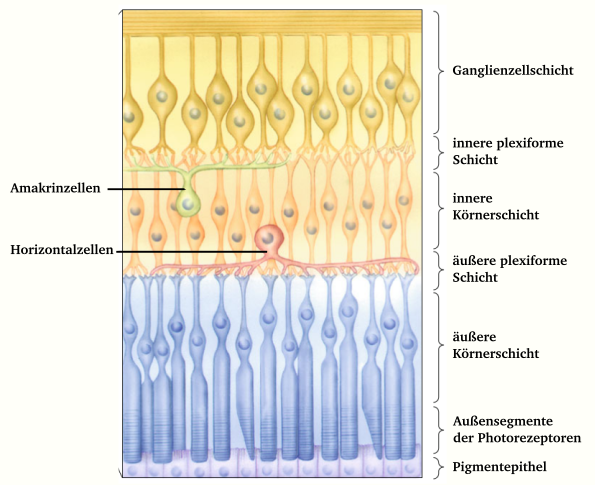
\includegraphics{pictures/visual/retina.png}
    \caption[Schichten in der Retina]{\textbf{Schichten in der Retina}\\
    Das Licht geht von oben durch die einzelnen Schichten bis es von den Photorezeptoren wahrgenommen wird. \\
    Abbildung nach Neurowissenschaften, Baer \textsuperscript{\cite[10]{neurowissenschaften_baer}}}
    \label{fig:retina}
\end{figure}

Wie bereits kurz erwähnt nehmen die Photorezeptoren das Licht wahr und wandeln sie in neuronale Signale um. Das Signal wird über die Bipolarzellen an die Ganglienzellen weiter gegeben. Die Axone der Ganglienzellen ziehen zur Sehnervenpapille. Diese liegt etwas medial der Fovea und bildet den \textbf{Blinden Fleck} \index{Blinder Fleck}, da an dieser Stelle keine Photorezeptoren vorhanden sind. Die gebündelten Axone bilden den Sehnerv (CN II), den \textbf{Nervus opticus}. \index{Hirnnerven! N. opticus} 


\begin{comment}
Die Abb. 9.12 zeigt, dass die Netzhaut eine laminare Struktur besitzt: Die Zellen sind
in Schichten organisiert. Die Schichten sind scheinbar verkehrt herum angeordnet: Das
Licht muss vom Glaskörper durch die Ganglienzellen und Bipolarzellen, bevor es die
Photorezeptoren erreicht. Weil die Netzhautzellen über den Photorezeptoren relativ trans-
parent sind, ist die Bildverzerrung minimal, wenn das Licht sie durchdringt. Ein Grund
dafür, dass die umgekehrte Anordnung vorteilhaft ist, besteht darin, dass das Pigmente-
pithel, das unter den Photorezeptoren liegt, eine entscheidende Rolle bei der Erneuerung
der Photorezeptoren und Photopigmente spielt. Zusätzlich absorbiert das Pigmentepithel
sämtliches Licht, das die Netzhaut durchdringt. Dadurch minimiert es die Streuung des
Lichts innerhalb des Auges, die das Bild undeutlich machen würde. Viele nachtaktive Tie-
re wie Katzen und Waschbären besitzen unterhalb der Photorezeptoren eine reflektierende
Schicht, das sogenannte Tapetum lucidum. Diese reflektiert durch die Netzhaut einfallen-
des Licht wieder zu den Photorezeptoren zurück. Daher sind diese Tiere empfindlicher
für schwache Lichtintensitäten, allerdings auf Kosten einer verringerten Sehschärfe. Ein
interessanter Nebeneffekt dieses reflektierenden Tapetum lucidum zeigt sich, wenn man
solche nachtaktiven Tiere anleuchtet oder beim Fotografieren anblitzt: Auf verblüffende
Weise scheinen ihre Pupillen regelrecht zu leuchten (Abb. 9.13) – daher rührt auch die
Bezeichnung „Katzenauge“ für bestimmte Arten von Rückstrahlern im Straßenverkehr.
Die Zellschichten der Netzhaut werden nach ihrer Entfernung zum Inneren des Auges
benannt. Man sollte sich aber nicht verwirren lassen, indem man an den Kopf statt das
Auge denkt. Die Photorezeptoren bilden die äußerste Schicht der Retina, obwohl sie am
weitesten von der Frontseite des Auges entfernt und am tiefsten im Kopf liegen. Dement-
sprechend bildet die innerste Schicht die Ganglienzellschicht. Sie setzt sich aus den
Zellkörpern der Ganglienzellen zusammen. Nach außen hin folgen zwei weitere Schich-
ten, die die Zellkörper von Neuronen enthalten: die innere Körnerschicht, welche die
Zellkörper der Bipolarzellen, der Horizontalzellen und der Amakrinzellen enthält, und die
äußere Körnerschicht mit den Zellkörpern der Photorezeptoren.
Zwischen der Ganglienzellschicht und der inneren Körnerschicht befindet sich die innere
plexiforme Schicht („plexiform“ steht für ein dichtes Netzwerk von Verbindungen), die
die synaptischen Verbindungen zwischen den Bipolarzellen, den Amakrinzellen und den
Ganglienzellen enthält. Zwischen der inneren und der äußeren Körnerschicht liegt die äu-
ßere plexiforme Schicht, in der die synaptischen Verbindungen der Photorezeptoren mit den Bipolar- und Horizontalzellen liegen. Die abschließende Schicht der Außensegmente
der Photorezeptorzellen beinhaltet die lichtempfindlichen Strukturen der Netzhaut. Die Enden der Außensegmente sind in das Pigmentepithel eingebettet.
\end{comment}


\subsubsection*{Das Optische Chiasma und der Optische Trakt}

\begin{comment}
Explaination of the other twopathways in biologie of sensory systems chapter 18
\end{comment}

Der linke und rechte Sehnerv ziehen über den optischen Kanal in die Schädelhöhle. An der Basis des Gehirns, unterhalb des \textit{Tuber cinereum} des Hypothalamus, laufen die beiden Sehnerven zum \textbf{Chiasma opticum} \index{Chiasma opticum} zusammen. 
Im Chiasma opticum kreuzen die Nerven aus dem nasalen Bereich des Gesichtsfelds auf die andere Seite. Da nur ein Teil der Nerven auf die andere Seite kreuzt, wird diese Kreuzung \textbf{Semidecussation} \index{Semidecussation} genannt. \textsuperscript{\cite[15]{crossman2014neuroanatomy}} 

In Abbildung~\ref{fig:sehbahn_baer} ist die Sehbahn des Menschen abgebildet. Aufgrund der nach frontalen Augen beim Menschen überlappen die beiden Sehfelder stark. Da Ratten lateral liegende Augen haben, ist bei ihnen eine bessere Rundumsicht möglich aber das binokulare Gesichtsfeld ist kleiner (40~-~60\% Überlappung). \textsuperscript{\cite[30]{paxinos2014rat}}
Alles was auf der linken Gesichtsfeldhälfte abgebildet wird, wird auf der rechten Retinahälfte abgebildet und umgekehrt. Der linke und rechte Sehnerv, trägt die Informationen des gesamten Sehfeldes eines Auges bis zum Chiasma opticum. Dort kreuzen die Nerven aus dem nasalen Bereich der Retina auf die andere Seite. Danach verlaufen der linke und rechte Tractus opticus, \index{Tractus opticus} diese tragen dann nur noch die Informationen aus einer Gesichtsfeldhälfte (rechter Tractus - linke Gesichtsfeldhälfte und umgekehrt) bis ins Gehirn.


\begin{figure}[H]
    \centering
    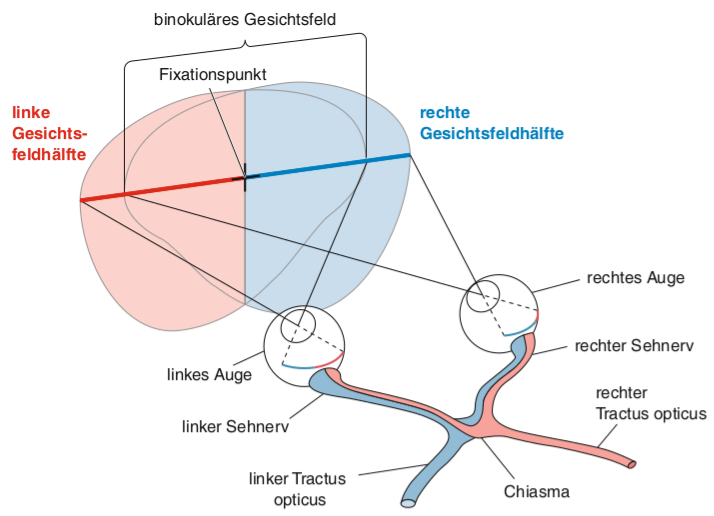
\includegraphics[width = 0.9\textwidth]{pictures/visual/Sehbahn.png}
    \caption[Die Sehbahn]{\textbf{Die Sehbahn}\\
    Die Sehbahn des Menschen mit dem Verlauf der Nervenbahnen und der Projektion der Informationen von der linken und rechten Gesichtsfeldhälfte.
    Abbildung nach Neurowissenschaften, Bear \textsuperscript{\cite[10]{neurowissenschaften_baer}}}
    \label{fig:sehbahn_baer}
\end{figure}

Im Chiasma opticum (Abb.~\ref{fig:optic_tract}~A) findet keine Verschaltung statt. Die Nervenbahnen kreuzen nur auf die andere Seite. Von da an werden die Sehbahnen, linker und rechter \textbf{Tractus opticus} \index{Tractus opticus} genannt. Der optische Trakt verläuft auf beiden Hemisphären um den \textit{Pedunculus cerebri} herum bis in den Nucleus geniculatum laterale im Thalamus (Abb.~\ref{fig:optic_tract}~B~-~E). \textsuperscript{\cite[15]{crossman2014neuroanatomy}}

\begin{figure}[H]
    \centering
    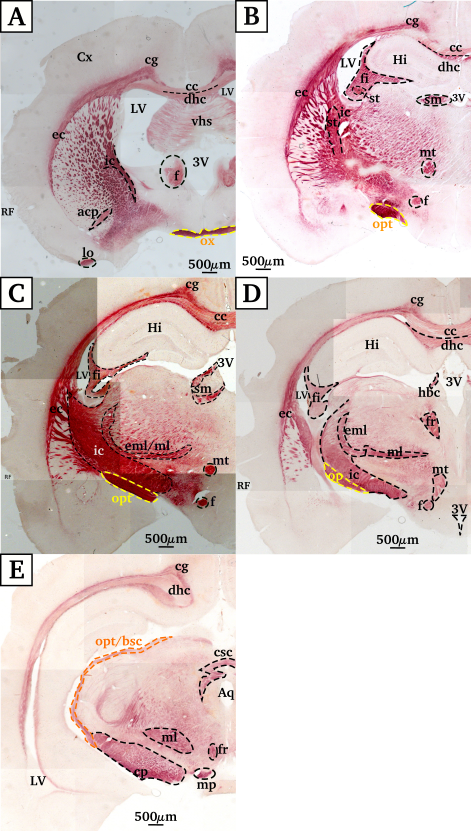
\includegraphics{pictures/visual/optic_tract.png}
    \caption[Das Optische Chiasma und der Optische Trakt]{\textbf{Das Optische Chiasma und der Optische Trakt}\\
    Der Verlauf des optischen Trakts vom optischen Chiasma bis zum Thalamus. \textbf{A}: F18-3 \textbf{B}: F20-3 \textbf{C}: F21-3 \textbf{D}: F23-3 \textbf{E}: F26-2}
    \label{fig:optic_tract}
\end{figure}

\subsubsection*{Beschriftung und Kürzel}

\begin{table}[H]
\begin{tabular}{llcll}
           & 3V  & -          & dritter Ventrikel                                                       & \multicolumn{1}{c}{\textbf{}} \\
\textbf{A} & acp & -          & Commissura anterior, posteriorer Teil                                   & \multicolumn{1}{c}{}          \\
\textbf{}  & Aq  & -          & Aquädukt, Aqueductus mesencephali, Aquaeductus cerebri                  & \multicolumn{1}{c}{}          \\
\textbf{B} & bsc & -          & Brachium colliculi superioris                                           & \multicolumn{1}{c}{}          \\
\textbf{C} & cc  & -          & Corpus callosum                                                         & \multicolumn{1}{c}{\textbf{}} \\
\textbf{}  & cg  & -          & Cingulum                                                                & \multicolumn{1}{c}{\textbf{}} \\
\textbf{ } & cp  & -          & Pedunculus cerebri, Kleinhirn-Pedunkel                                  & \multicolumn{1}{c}{\textbf{}} \\
\textbf{ } & csc & -          & Commissura colliculi superioris                                         & \multicolumn{1}{c}{\textbf{}} \\
\textbf{}  & Cx  & -          & Cortex                                                                  & \multicolumn{1}{c}{}          \\
\textbf{D} & dhc & -          & dorsale Hippocampus-Kommissur                                           & \multicolumn{1}{c}{}          \\
\textbf{E} & ec  & -          & Capsula externa                                                         &                               \\
\textbf{ } & eml & -          & Lamina medullaris lateralis, external medullary lamina                  &                               \\
\textbf{F} & f   & -          & Fornix                                                                  &                               \\
\textbf{}  & fi  & -          & Fimbria                                                                 &                               \\
\textbf{}  & fr  & -          & Fasciculus retroflexus                                                  &                               \\
\textbf{H} & hbc & -          & Commissura habenularum                                                  &                               \\
\textbf{}  & Hi  & -          & Hippocampus                                                             &                               \\
\textbf{I} & ic  & -          & Capsula interna                                                         &                               \\
\textbf{L} & lo  & -          & lateraler olfaktorischer Tract, tractus olfactorius lateralis           &                               \\
\textbf{}  & LV  & -          & lateraler Ventrikel                                                     &                               \\
\textbf{M} & ml  & -          & medialer Lemniscus                                                      &                               \\
\textbf{}  & mp  & -          & Mammilar-Pedunkel                                                       &                               \\
\textbf{}  & mt  & -          & mammilothalamischer Trakt                                               &                               \\
\textbf{O} & opt & -          & optischer Trakt, Tractus opticus                                        &                               \\
\textbf{}  & ox  & -          & Chiasma opticum                                                         &                               \\
\textbf{R} & RF  & -          & Fissura rhinalis                                                        &                               \\
\textbf{S} & sm  & -          & Stria medullaris thalami                                                &                               \\
\textbf{}  & st  & -          & Stria terminalis                                                        &                               \\
\end{tabular}
\end{table}

\begin{comment}
Its laterally placed eyes provide it
with a panoramic view, with a binocular overlap of
40–60 o in front of, and above, the animal
\textsuperscript{\cite[30]{paxinos2014rat}}

The axons of retinal ganglion cells assemble at the optic disc
and pass into the optic nerve, which enters the cranial cavity
through the optic canal. The two optic nerves converge to
form the optic chiasm on the base of the brain (Fig. 15.5).
The chiasm lies immediately rostral to the tuber cinereum
of the hypothalamus and between the terminating internal
carotid arteries. In the chiasm, axons derived from the nasal
halves of the two retinae decussate and pass into the
contralateral optic tract, while those from the temporal
hemiretinae remain ipsilateral. The optic tracts diverge away
from the chiasm and pass round the cerebral peduncle to
terminate mainly in the lateral geniculate nucleus (within the
lateral geniculate body) of the thalamus. \textsuperscript{\cite[15]{crossman2014neuroanatomy}}

Bild aus dem Baer Kapitel 10

Die Namen der Bahnen
Semidecussiation
Projektion welcher Hälfte auf welche Seite

Projelktion in den LGN

The axons of
retinal neurons (ganglion cells) carry information from each
visual hemifield along the optic nerve up to the optic chi-
asm, where fibers from the nasal hemiretina cross to the
opposite hemisphere. Fibers from the temporal hemiretina
stay on the same side, joining the fibers from the nasal
hemiretina of the contralateral eye to form the optic tract.
The optic tract carries information from the opposite visual
hemifield originating in both eyes and projects into the
lateral geniculate nucleus.
\end{comment}

\newpage
\subsubsection*{Der Corpus geniculatum laterale}

Der \textbf{Corpus geniculatum laterale} (\textbf{LGN}) \index{Corpus geniculatum laterale} liegt im posterioren Teil des Thalamus und gehört zu den Nuclei des Kniehöckers (Abb.~\ref{fig:LGN}). \textsuperscript{\cite[12]{crossman2014neuroanatomy}} Im LGN terminieren die Ganglienzellen der kontralateralen Gesichtshälfte, beziehungsweise aus der ipsilateralen Netzhauthälften beider Retinae. Die Informationen aus den Ganglionzellen werden im LGN unter Einflussnahme des visuellen Cortex verarbeitet.
\textsuperscript{\cite[8.1]{trepel2011neuroanatomie}}

\begin{figure}[H]
    \centering
    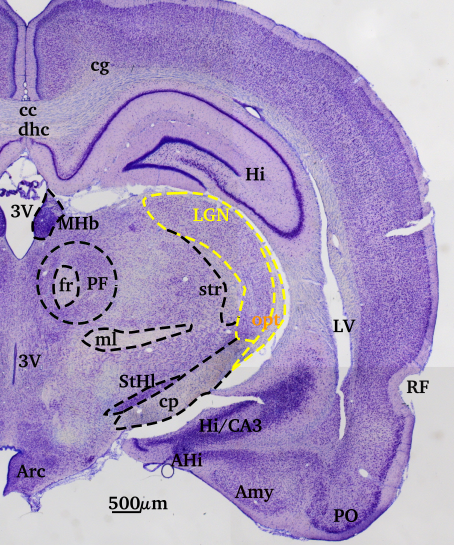
\includegraphics{pictures/visual/LGN.png}
    \caption[Corpus geniculatum laterale]{\textbf{Corpus geniculatum laterale}\\
    Nissel-Färbung (N20-4)}
    \label{fig:LGN}
\end{figure}

Der LGN hat bei Altweltaffen und dem Menschen sechs Schichten. 
In Abbildung~\ref{fig:schichtung-LGN} sieht man die sechs Schichten die wie Hüte gestapelt den Corpus geniculatum laterale bilden. In Schicht 1 und 2 terminieren die M-Ganglienzellen, wobei in Schicht 1 die contralateralen Neurone terminieren und in Schicht 2 die der ipsilateralen Seite. Sie geben die Informationen an die magnozellulären LGN-Zellen weiter. Die Axone der P-Ganglienzellen terminieren in Schicht 3 bis 6 an den parvozellulären LGN-Zellen, auch hier ist der Input aus den Augen streng getrennt. Es ergibt sich folgende Reihenfolge; Schicht 3: ipsilateral; Schicht 4: contralateral; Schicht 5: ipsilateral; Schicht 6: contralateral.
Zwischen den Schichten liegen die Schichten der konizellulären LGN-Zellen. Sie bekommen Input aus den nonM-nonP-Ganglienzellen. \textsuperscript{\cite[9.7]{heldmaier2003tierphysiologie}}


\begin{figure}[H]
    \centering
    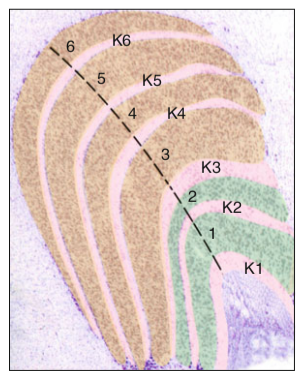
\includegraphics{pictures/visual/LGN_baer.png}
    \caption[Schichtung des LGN]{\textbf{Schichtung des LGN}\\
    Die sechs Schichten des Corpus geniculatum laterale des Menschen. Schicht 1 und 2 bekommen Input aus den M-Ganglienzellen, Schicht 3~-~6 aus den P-Ganglionzellen und die Schichten dazwischen aus den nonM-nonP-Ganglienzellen. Die Zellen des LGN in den zwischen Schichten werden konikuläre Zellen (K1~-~K6) genannt.\\
    Abbildung nach Neurowissenschaften, Baer \textsuperscript{\cite[10]{neurowissenschaften_baer}}}
    \label{fig:schichtung-LGN}
\end{figure} 

Aufgrund der Funktion der M-Ganglienzellen haben die magnozellulären LGN-Neurone ebenfalls farbenblinde rezeptive Felder. Sie reagieren vor allem auf Bewegungs-Stimmuli im rezeptiven Feld. In den Schichten 3 bis 6 bekommen die parvozellulären LGN-Neurone eingehende Informationen aus den farbsensitiven P-Ganglienzellen. Die rezeptiven Felder der LGN-Neurone in Schicht 3 und 4 sind blau/gelbe OFF~-~ON Felder, während die Neurone in Schicht 5 und 5 rot/grüne ON~-~OFF Felder sind. \textsuperscript{\cite[18]{smith2008biology}}

Die Neurone des Corpus geniculatum laterale ziehen über die Seilstrahlung (\textbf{Radiatio optica}) \index{Radiatio optica} in den visuellen Cortex. \textsuperscript{\cite[8.1]{trepel2011neuroanatomie}}

\begin{comment}
Lage des LGN

The geniculate nuclei are located near the posterior pole of
the thalamus, ventral to the pulvinar. Here, they form small
eminences on the surface, known as the geniculate bodies.
The lateral geniculate nucleus is a part of the visual system
and receives further discussion in Chapter 15. It is the site
of termination of the optic tract, which carries the axons of
retinal ganglion cells. As a result of hemidecussation of optic
nerve fibres in the optic chiasm, each lateral geniculate
nucleus receives axons that have originated from the
ipsilateral temporal hemiretina and the contralateral nasal
hemiretina. Each nucleus thus receives visual information
relating to the contralateral half of the visual field. The lateral
geniculate nucleus sends fibres, via the retrolenticular part of
the internal capsule and the optic radiation, to the primary
visual cortex of the occipital lobe.
\textsuperscript{\cite[12]{crossman2014neuroanatomy}}

Aufbau beim Menschen nicht gleich der Ratte

Seine wichtigsten Afferenzen erhält dieser Kern über den
Tractus opticus, der die visuelle Information der kontralatera-
len Gesichtsfeld.hälfte, d. h. also die der ipsilateralen Netzhaut-
hälften beider Retinae führt. Die Information wird hier unter
afferenter Einflussnahme visueller Kortexareale verschaltet
und über die Seilstrahlung (Radiatio optica) der okzipitalen
Sehrinde zugeleitet (zur Sehbahn als Ganzes >- Kap. 9.8.1).
Das Corpus geniculatum laterale besteht histologiscll aus seclls
Schicllten: zwei basal gelegene großzellige (magnozelluläre) und vier darüber liegende kleinzellige (parvozelluläre) Schich-
ten. Dies hat bei der funktionellen Teilung der Sehbahn in ein
magno- wtd parvozelluläresSystem Bedeutung ( > Kap. 9.9.1)
\textsuperscript{\cite[8.1]{trepel2011neuroanatomie}}

Das dorsale Corpus geniculatum laterale (LGN) der Altweltaffen
und seine retinatop geordneten S chichten. Jede Schicht
Parasol-Ganglienzellen
wird nur vom ipsi- (i) oder kontralateralen (c) Auge in-
K5
nerviert. Bei Primaten enden die midget-Ganglienzellen
M2i magno-
in den parvozellulären Schichten P3-P6, und die Para-
M1c zellulär
sol-Ganglienzellen in den magnozellulären Schichten Ml
und M2. Die Eingänge in die dazwischen gelagerten ko-
niozellulären Schichten (Kl-K6) sind noch unklar. Die
"bistratified"-Ganglienzellen (kodieren die Farbe blau)
enden in Schicht K3 und K4 (blau) \textsuperscript{\cite[9.7]{heldmaier2003tierphysiologie}}

Funktion

In
layers 1 and 2 the receptive fields have a ‘colour
blind’ centre–surround organization similar to the
centre–surround fields of alpha ganglion cells. These
cells are highly sensitive to motion in their RFs. Re-
ceptive fields with similar characteristics can, indeed,
be found throughout the LGNd’s six layers. But in
the upper layers, as would be expected from the par-
vocellular input, the cells are mostly responsive to
colour. Layers 3 and 4 are dominated by OFF-centre
blue/yellow (or, better, blue/red + green) opponent
cells, whereas in layers 5 and 6 ON-centre red/green
opponent cells predominate. The narrow diameter
slowly-conducting axons of the W cells project to
the parvocellular layers.
\textsuperscript{\cite[18]{smith2008biology}}

Zelltypen

Burke and Sefton (1966a) classified cells recorded in
DLG as P (principal or relay) and I (interneuronal) on
the basis of electrical properties.
\textsuperscript{\cite[30]{paxinos2014rat}}

These nuclei (or bodies) are located in the posterior
part of the thalamus. Their dorsal parts (LGNd) have
a distinctive laminated structure (Figure 18.3). This
has often been likened to a stack of hats, one inside
the other. In primates there are six layers of cells sep-
arated by bands of fibres. It is here that the optic
nerve fibres (the axons, it will be remembered, of the
retinal ganglion cells) terminate. Because of the par-
tial decussation described above (Figure 18.2), nerve
fibres come from the temporal half of the ipsilateral
eye and the nasal half of the contralateral eye. The
LGNd maintains a strict segregation of these fibres.
The fibres from the contralateral eye terminate in
layers 1, 4 and 6, whilst those from the ipsilateral
eye terminate in layers 2, 3 and 5. The fibres make
synapses with a second set of neurons which, form-
ing the optic radiations, carry the visual information
on to the primary visual cortex.
How precise the connectivity is remains a matter of
debate. It is known, however, that optic nerve fibres
divide into up to six branches, making synapses with
six separate neurons in the same layer of the LGNd.
One geniculate neuron, vice versa, may synapse with
more than one incoming optic nerve fibre. Connector
neurons are also present running between neurons in
a single lamina. The separation of the input from
the two eyes is, however, maintained. Finally, there
is a significant innervation from the visual cortex
(corticofugal innervation). This has a powerful feed-
back function. The LGNd cannot, therefore, be con-
sidered a simple junction box.
Let us now return to the fibres in the optic nerve
and tract. We noted in Section 17.2.8 that these fi-
bres could be classified into two major and one mi-
nor group: magnocellular (M) fibres, parvocellular
(P) fibres and W fibres. The M pathway, which car-
ries information mostly pertaining to movement of
he visual image, terminates in layers 1 and 2 of the
LGNd (the magnocellular layers) whilst the P path-
way, mostly concerned with colour information, ter-
minates in layers 3, 4, 5 and 6 (the parvocellular
layers). These cells can be investigated by micro-
electrode recording. As would be expected, they re-
spond to illumination of appropriate patches of the
retina. These patches are consequently said to con-
stitute the receptive fields of the geniculate cells. 
In
layers 1 and 2 the receptive fields have a ‘colour
blind’ centre–surround organization similar to the
centre–surround fields of alpha ganglion cells. These
cells are highly sensitive to motion in their RFs. Re-
ceptive fields with similar characteristics can, indeed,
be found throughout the LGNd’s six layers. But in
the upper layers, as would be expected from the par-
vocellular input, the cells are mostly responsive to
colour. Layers 3 and 4 are dominated by OFF-centre
blue/yellow (or, better, blue/red + green) opponent
cells, whereas in layers 5 and 6 ON-centre red/green
opponent cells predominate. The narrow diameter
slowly-conducting axons of the W cells project to
the parvocellular layers.
\textsuperscript{\cite[18]{smith2008biology}}
\end{comment}

\subsubsection*{Der visuelle Cortex}

Der visuelle Cortex umfasst den primären und sekundären visuellen Cortex und übergeordneter visueller Cortexareale. Der visuelle Cortex liegt im Okzipitallappen im caudalen Bereich des Großhirns. \textsuperscript{\cite[15]{crossman2014neuroanatomy}} 


\subsubsection*{Der primäre visuelle Cortex}

Der \textbf{primäre visuelle Cortex} (\textbf{V1}) \index{Cortex! visueller, V1} umfasst das Brodmann-Areal 17. Er liegt auf der medialen Oberfläche der Hemisphäre und umgibt den Sulcus calcarinus\index{Sulcus! calcarinus}, wie in Abbildung~\ref{fig:V1} zu sehen ist. \textsuperscript{\cite[10]{neurowissenschaften_baer}} 
Der primäre visuelle Cortex unterscheidet sich vom Rest des Neocortex durch seine makroskopisch sichtbare Streifen. Diese entstehen weil der Cortex mit Streifen (Gennari-Streifen) aus myelinisierten Fasern, die parallel zur Oberfläche in Schicht 4 verlaufen, durchzogen ist. Aus diesem Grund nennt man diesen Bereich des Cortex auch Area striata. \textsuperscript{\cite[18]{smith2008biology}}

Die Fasern aus dem ipsilateralen LGN ziehen in den ipsilateralen primären visuellen Cortex und terminieren in Schicht 4. Die eingehenden Informationen sind in dieser Schicht streng monokular getrennt. Die biokulare Verarbeitung findet in den anderen Schichten (II-VI) statt. Eine Hemisphäre in V1 verarbeitet etwas mehr als die Hälfte des Sehfeldes. Die Sehfelder überlappen an der vertikalen Mittellinie. \textsuperscript{\cite[25]{kandel2013principles}} 
Wie in Abbildung~\ref{fig:V1} zu sehen ist, ist die Repräsentation der einzelnen Bereichen des Sehfeldes im Cortex nicht der selben Größe entsprechend die die auf der Retina einnehmen. Die Bereiche der Fovea und um die Fovea herum nehmen mehr cortikale Fläche ein als die Randbreiche der Retina. Die corticale Flächengröße die Input aus einem Sehbereich von einem Grad bekommt, wird durch den Magnifikationsfaktor berechnet und nimmt zur Fovea hin ab. \textsuperscript{\cite[25]{kandel2013principles}}
\\
\\

\begin{comment}
Eingehende Informationen aus dem LGN gehen in Schicht 4. 
Aufbau der Schichten und monokular in Schicht 4 und biokular in Schicht 2 und 3

A major fiber bundle called the corpus callosum
connects the two hemispheres, transmitting information
across the midline. The primary visual cortex in either
hemisphere represents slightly more than half the visual
field, with the two hemifield representations overlap-
ping at the vertical meridian. One of the functions of the
corpus callosum is to unify the perception of objects
spanning the vertical meridian by linking the cortical
areas that represent opposite hemifields.
\textsuperscript{\cite[25]{kandel2013principles}}

Before turning to these extrastriate cortices, it is
important to remind ourselves that, as in the other
sensory systems considered in this book, the sensory
surface, in this case the retina, is displayed as a non-
isomorphous map in the sensory cortex, in this case
the primary visual cortex. This map is shown in Fig-
ure 18.19. As noted above, the aggregate receptive
fields in the fovea are the smallest in extent, hence
far more of the visual cortex is devoted to them than
to other parts of the retina. It can be seen from the
figure that the upper parts of the retina are mapped in
the lower bank of the calcarine fissure and vice versa.
It must be remembered that, because of the optics of
the eye, the upper part of the retina corresponds to
the lower part of the visual field and vice versa. The
cortex devoted to the fovea is almost as large as all
the rest (Figure 18.19) and, indeed, extends out on
to posterior surface of the occipital lobe. It is from
this map that fibres carrying processed information
about the visual scene are directed onwards to the
extrastriate cortices \textsuperscript{\cite[18]{smith2008biology}}

Eigentliche Funktion des V1

rezeptive Felder 
They soon showed that when a bar stimulus, or an
edge, at a particular orientation, was either flashed on
or swept across an appropriate part of the retina, the
cortical cell would respond with a burst of activity
\textsuperscript{\cite[18]{smith2008biology}}
Further work showed that, in the macaque striate
cortex, some 70–80\% of all the cells have this orienta-
tion specificity. Note that it is only movement of the
bar stimulus across the field which elicits a response.
Stationary stimuli have little effect. It was also found
that in some 30\% of the cells, the direction in which
the bar was swept was significant.

Blobs und Interblobs

To everyone’s surprise, cytochrome oxidase appeared to
be localized in a regular series of ‘blobs’, which are
particularly obvious in layers 2 and 3 of the stri-
ate cortex. These blobs are about 0.5 mm in diam-
eter, separated from each by so-called ‘interblob’
regions about 0.25 mm across. For some years no
one took much notice of this unexpected finding.
Then, in 1981, Hubel and Livingstone examined the
blobs with the microelectrode. It was found that,
far from being composed of orientation selector
cells, the blobs consisted of cells with concentric
centre–surround fields responsive to colour. \textsuperscript{\cite[18]{smith2008biology}}
\end{comment}


\begin{figure}[H]
    \centering
    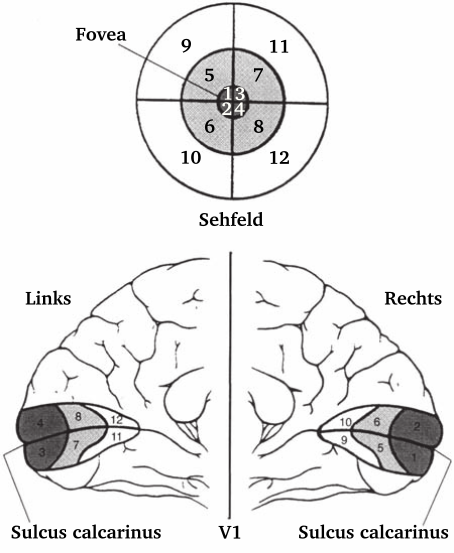
\includegraphics[width = 0.6\textwidth]{pictures/visual/V1.png}
    \caption[Der primäre visuelle Cortex]{\textbf{Der primäre visuelle Cortex}\\
    Die Abbildung des Sehfeldes auf dem primären visuellen Cortex. Das Sehfeld kann in vier Quadranten eingeteilt werden. Der erste und zweite Quadrant (linkes Sehfeld) werden auf der rechten Hemisphäre abgebildet. Der dritte und vierte Quadrant wird auf der linken Hemisphäre abgebildet. Die Sehbereiche näher zur Fovea (1~-~4) werden im caudalen Bereich von V1 abgebildet, wohingegen die Sehfelder distal zur Fovea (9~-~12) im rostralen Bereich abgebildet werden.\\
    Abbildung nach Biology of Sensory Systems, Smith \textsuperscript{\cite[18]{smith2008biology}}}
    \label{fig:V1}
\end{figure}


\noindent Wie bereits erwähnt verarbeiten die anderen Schichten im primären visuellen Cortex die Informationen aus beiden Augen. Der Aufbau dieser Schichten ist aber weiterhin sehr geordnet. Die rezeptiven Felder in diesen Schichten sind nicht mehr rund wie in den vorherigen Verarbeitungszentren sondern rechteckig. Die rezeptiven Felder verarbeiten in V1 Balkenstimuli mit einer gewissen Orientierung im rezeptiven Feld oder reagieren auf nur eine bestimmte Richtung aus der der Stimulus durch des rezeptive Feld fährt. Die rezeptiven Felder reagieren in V1 nur noch selten auf stationäre Stimuli, sondern immer auf Bewegung im rezeptiven Feld. \textsuperscript{\cite[18]{smith2008biology}}

Rezeptive Felder mit einer bestimmten Richtung befinden sich in einer Reihe im Cortex. Diese bilden dann sogenannte Orientierungssäulen. Orthogonal dazu verlaufen in Schicht 4 die Dominanzsäulen in den jeweils nur die rezeptiven Felder eines Auges liegen. \textsuperscript{\cite[10]{neurowissenschaften_baer}} 
In den Schichten 2~\&~3 verlaufen auch noch sogenannte Cytochromoxidase-Blobs. In diesen liegen konzentrische rezeptive Felder die auf Farbstimuli reagieren. \textsuperscript{\cite[18]{smith2008biology}}

\begin{comment}
Lage

The primary visual cortex is, how-
ever, distinguished from other parts of the neocortex
by the presence of a strongly developed strip of myeli-
nated fibres running parallel to the pial surface in
layer 4 known as the stripe of Gennari (hence the
name, striate cortex)
\textsuperscript{\cite[18]{smith2008biology}}

The primary visual cortex is located predominantly on the
medial surface of the hemisphere in the region above and
below the calcarine sulcus. Surrounding this area, the rest of
the occipital lobe constitutes the visual association cortex. It is
concerned with interpretation of visual images, recognition,
depth perception and colour vision.
\textsuperscript{\cite[15]{crossman2014neuroanatomy}}

Das CGL hat ein einziges axonales Projektionsgebiet: die primäre Sehrinde. Wie bereits
in Kap. 7 dargestellt wurde, kann der Cortex, basierend auf seinen Verknüpfungen und
seiner Cytoarchitektur, in verschiedene Areale eingeteilt werden. Die primäre Sehrinde
entspricht dem Brodmann-Areal 17 und ist im Hinterhauptslappen des Großhirns loka-
lisiert. Ein Großteil von Areal 17 liegt auf der medialen Oberfläche der Hemisphäre und
umgibt den Sulcus calcarinus (Abb. 10.10). Weitere Bezeichnungen der Sehrinde sind V1
und striärer Cortex. \textsuperscript{\cite[10]{neurowissenschaften_baer}}

Die primäre Sehrinde kleidet die Wand des Sulcus calcarinus
aus, greift auf die mediale Fläche des Okzipitallappens tmd auf
den Okzipitalpol über und nimmt die Area 17 nach Brodmann
ein (>- Abb. 9.33, 1). Da sie in ihrer grauen Substanz einen be-
reits makroskopisch sichtbaren weißen Streifen (Getmari- oder
Vicq-d'Azyr-Streifen) aufweist, der parallel zur Oberfläche ver-
läuft, wird sie auch Area striata gena~mt ( >- Abb. 9.49b, 6).
Die Area 17 ist als primäre Sehrinde (primärer visueller Kor-
tex) der zerebrale Ort der Bewusstwerdung der visuellen Impulse
aus der Retina. Eine Interpretation bzw. ein erkennendes Zuord-
nen des visuellWahrgenommenen erfolgt hier aber noch nicht.
\textsuperscript{\cite[9.8]{trepel2011neuroanatomie}}

\end{comment}

\subsubsection*{Höhere visuelle Verarbeitungszentren und coritco-corticale Verbindungen}

eyond the striate
cortex lie the extrastriate areas, a set of higher-order
visual areas that are also organized as neural maps of
the visual field. The preservation of the spatial arrange-
ment of inputs from the retina is called retinotopy, and
a neural map of the visual field is described as retino-
topic or having a retinotopic frame of reference.

From there
information is transmitted over two major pathways.
A ventral pathway into the temporal lobe carries informa-
tion about what the stimulus is, and a dorsal pathway into
the parietal lobe carries information about where the stim-
ulus is, information that is critical for guiding movement.
\textsuperscript{\cite[25]{kandel2013principles}}

V2
vllt ganzkurz die zwei generellen Projektionswege
    temporallappen
    parietallappen
    
\begin{figure}[H]
    \centering
    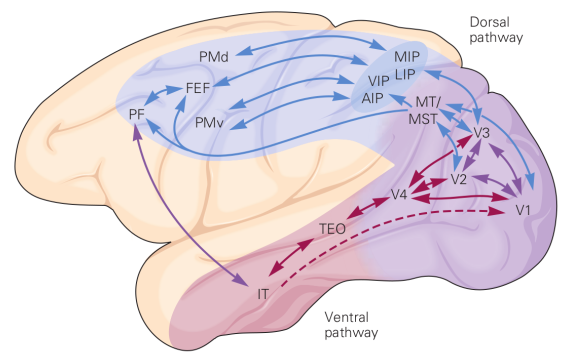
\includegraphics{pictures/visual/visual_Cortex.png}
    \caption[Visuelle Verarbeitungszentren im Cortex]{\textbf{Visuelle Verarbeitungszentren im Cortex}\\
    Abbildung nach Principles of Neural Science, Kandel \textsuperscript{\cite[27]{kandel2013principles}}}
    \label{fig:visual_pathway_cortex}
\end{figure}
















\begin{comment}
\begin{itemize}
    \item eye
    \begin{itemize}
        \item kurzer überblick über die entwicklung des auges in der embryonal entwicklung retina aus dem diencephalon
        \item auf grund der evolutionären Entwicklunf ein "inverted" auge wesswegen die retina und die photorezeptoren nach innen weg vom licht gerichtet sind
        \item formung der retina: \cite{smith2008biology} p.287
        \item retinale zellen Stäbchen und zäpfchen und dann bipolar zellen und Ganglienzellen 
        \item vllt was zu den rezeptifen feldern
    \end{itemize}
    \item visual pathway
    \begin{itemize}
        \item 3 verschiedene wege ( vorlesung von oswald IN)
        \item wie heißen die von führen sie hin und wir konzentrieren uns auf einen zentralen und warum
    \end{itemize}
    \item optic nerve von der Retina zum Chiasma opticum
    \item Optic chiasm    \index{Optic chiasm}
    \begin{itemize}
        \item Semidecussation  \index{Decussation!Semi-}
        \item ganglienzellen von der nasalen/medialen seite des auges kreuzen am optic chiasm auf die andere seite des gehirns wärend die laterale seite des auges auf der selben seite weiter projezieren
        ßitem keine verschaltung im optischen chiasma sondern nur eine kreuzung der ganglien zellen
        \item danach optic tract
    \end{itemize}
    \item Optic tract \index{Optic tract}
    \item LGN: nicht gestreift, hinterer Teil das Thalamus \index{Thalamus}, auf Höhe des superior colliculus \index{SC!Superior culliculus}
    \begin{itemize}
        \item lateral am Diencephalon \index{Diencephalon} vorbei
        \item posteriorer part des thalamus
        \item aufbau des LGN unterschied zwischen primaten (6 Schichten) und Ratten bzw. Schafen
        \item kurz was zur funktion der verschaltung auf der ebene ( vllt etwas zu den rezeptive fields aber dann auch schon auf der ebene der retina erwähnen)
        \item von LGN über die optic radiation (welche nicht in den schnitten sichtbar ist) ruaf in den neocortex und in V1 
    \end{itemize}
    \item Magnifikationsfaktor = Dichte der Zellen und wie sie verschaltet sind
    \\
\end{itemize}
\end{comment}


\subsection{(Riechbahn)}
\begin{itemize}
    \item vom olfactorischen bulb über den olfactorischen trakt zu einerm der ältesten teile des neocortex zum Pyriformen lappen
    \item weitere neuronen führen dann zum thalamus un die weitern stränge dann in den orbitofrontal lobe \cite{smith2008biology} 
    \item eventuell Dopaminerge Bilder
\end{itemize}

%%%%%%%%%%%%%%%%%%%%%%%%%%%%%%%%%%%%%%%%%%%%%%%%%%%%%%%%%%5%%
% Bibliography

\newpage
\bibliographystyle{abbrv}
\bibliography{references}

%%%%%%%%%%%%%%%%%%%%%%%%%%%%%%%%%%%%%%%%%%%%%%%%%%%%%%%%%%%%%
% Index
\printindex

\end{document}


